%! Author = sebash
%! Date = 6/14/22

\documentclass{article}
\usepackage{blindtext}
\usepackage{amsmath, amssymb}
\usepackage[makeroom]{cancel}
\usepackage{tikz}
\usetikzlibrary{calc,shapes, arrows}
\usepackage{sectsty}
\usepackage{amssymb}


\newcommand{\tikzmark}[1]{\tikz[overlay,remember picture] \node (#1) {};}
\newcommand{\DrawBox}[2]{%
    \begin{tikzpicture}[overlay,remember picture]
        \draw[->,shorten >=5pt,shorten <=5pt,out=70,in=130,distance=0.5cm,#1] (MarkA.north) to (MarkC.north);
        \draw[->,shorten >=5pt,shorten <=5pt,out=50,in=140,distance=0.3cm,#2] (MarkA.north) to (MarkB.north);
    \end{tikzpicture}
}

\newcommand{\DrawBoxThree}[3]{%
    \begin{tikzpicture}[overlay,remember picture]
        \draw[->,shorten >=5pt,shorten <=5pt,out=70,in=130,distance=0.5cm,#1] (MarkA.north) to (MarkC.north);
        \draw[->,shorten >=5pt,shorten <=5pt,out=50,in=140,distance=0.3cm,#2] (MarkA.north) to (MarkB.north);
        \draw[->,shorten >=5pt,shorten <=5pt,out=90,in=120,distance=0.7cm,#3] (MarkA.north) to (MarkD.north);
    \end{tikzpicture}
}
\title{Sebastian Campos Homework}

\DeclareMathSizes{12}{30}{16}{12}

\begin{document}
    \maketitle
    \noindent
    \section*{2.1 5 to 29 odd}
    \subsection*{5.}
        \begin{align*}
            & \tikzmark{MarkA}15(y\tikzmark{MarkB}-9\tikzmark{MarkC})\DrawBox{black}{black} = -60 \\
            & 15y - 120 = -60 \\
            & 15y \hspace{.2cm}\cancel{-120} = \cancelto{60}{-60} \\
            &\hspace{.6cm} + 120 \hspace{.5cm} + 120 \\
            & 15y = 60 \\
            & y = \frac{60}{15} \\
            & \boxed{y = 4}
        \end{align*}

    \subsection*{7.}
        \begin{align*}
            & - (w - 12) = 30 \\
            & \tikzmark{MarkA}-(w\tikzmark{MarkB} - 12\tikzmark{MarkC})\DrawBox{black}{black} = 30 \\
            & -w + 12 = 30 \\
            & -w \hspace{.2cm}\cancel{+ 12} = \cancelto{18}{30} \\
            &\hspace{.6cm} - 12 \hspace{.4cm} - 12 \\
            & -w = 18 \\
            & \boxed{w = -18}
        \end{align*}

    \subsection*{9.}
    \begin{align*}
        & 51 + 5(4 - q) = 56 \\
        & 51 + \tikzmark{MarkA}5 (4\tikzmark{MarkB} - q\tikzmark{MarkC})\DrawBox{black}{black} = 56 \\
        & 51 + 20 -5q = 56 \\
        & 71 -5q = 56 \\
        & \hspace{.25cm}\cancel{71} - 5q = \cancelto{-15}{56} \\
        & - 71 \hspace{.8cm} - 71 \\
        & -5q = -15\\
        & q = \frac{-15}{-5} \\
        & \boxed{q = 3}
    \end{align*}

    \subsection*{11.}
    \begin{align*}
        & 3(10 -2x) + 54 = 0 \\
        & \tikzmark{MarkA}3 (10\tikzmark{MarkB} - 2x\tikzmark{MarkC})\DrawBox{black}{black} + 54 = 0 \\
        & 30 - 6x + 54 = 0 \\
        & - 6x + 84 = 0 \\
        & -6x + \cancel{84} = \cancelto{-84}{0} \\
        & \hspace{.8cm} -84 -84 \\
        & -6x = -84 \\
        & x = \frac{-84}{-6} \\
        & \boxed{x = 14}
    \end{align*}

    \subsection*{13.}
    \begin{align*}
        & \frac{2}{3}(9c - 3) = 22 \\
        & \tikzmark{MarkA}\frac{2}{3} (9c\tikzmark{MarkB} - 3\tikzmark{MarkC})\DrawBox{black}{black} = 22 \\
        & 6c - 2 = 22 \\
        & 6c \cancel{- 2} = \cancelto{24}{22} \\
        & \hspace{.2cm}+ 2\hspace{.2cm}+ 2 \\
        & 6c = 24 \\
        & c = \frac{24}{6} \\
        & \boxed{c = 4}
    \end{align*}

    \subsection*{15.}
    \begin{align*}
        & \frac{1}{5}(15c + 10) = c + 7 \\
        & \tikzmark{MarkA}\frac{1}{5} (15c\tikzmark{MarkB} + 10\tikzmark{MarkC})\DrawBox{black}{black} = c + 7 \\
        & 3c + 2 = c + 7 \\
        & 3c \cancel{+ 2} = c + \cancelto{5}{7} \\
        & \hspace{.2cm}- 2\hspace{.8cm}- 2 \\
        & 3c = c + 5 \\
        & \cancelto{2c}{3c} = \cancel{c} + 5 \\
        & 2c = 5 \\
        & \frac{2c}{2} = \frac{5}{2} \\
        & \boxed{c = \frac{5}{2}}
    \end{align*}

    \subsection*{17.}
    \begin{align*}
        & 3(4n -1) - 2 = 8n + 3 \\
        & \tikzmark{MarkA}3 (4n\tikzmark{MarkB} - 1\tikzmark{MarkC})\DrawBox{black}{black} = 8n + 3 \\
        & 12n - 3 - 2 = 8n + 3 \\
        & 12n - 5 = 8n + 3 \\
        & 12n \cancel{- 5} = 8n + \cancelto{8}{3} \\
        & \hspace{.4cm}+ 5 \hspace{1cm}+ 5 \\
        & 12n = 8n + 8 \\
        & \cancelto{4n}{12n} = \cancel{8n} + 8 \\
        & - 8n \hspace{.6cm} -8n \\
        & 4n = 8 \\
        & \frac{4n}{4} = \frac{8}{4} \\
        & \boxed{n = 2}
    \end{align*}

    \subsection*{19.}
    \begin{align*}
        & 12 + 2(5 -3y) = -9(y - 1) - 2 \\
        & 12 + \tikzmark{MarkA}2 (5\tikzmark{MarkB} - 3y\tikzmark{MarkC})\DrawBox{black}{black} = -\tikzmark{MarkA}9 (y\tikzmark{MarkB} - 1\tikzmark{MarkC})\DrawBox{black}{black} - 2 \\
        & 12 + 10 - 6y = -9y + 9 - 2\\
        & 22 - 6y = -9y + 7\\
        & 22 \cancel{- 6y} = \cancelto{-3y}{-9y} + 7 \\
        & \hspace{.3cm}+ 6y \hspace{.4cm}+ 6y \\
        & 22 = -3y + 7 \\
        & \cancelto{15}{22} = -3y \cancel{+ 7} \\
        & -7 \hspace{1.2cm} -7 \\
        & 15 = -3y \\
        & \frac{15}{-3} = \frac{-3y}{-3} \\
        & -5 = y \\
        & \boxed{y = -5}
    \end{align*}

    \subsection*{21.}
    \begin{align*}
        & 5 + 6(3s - 5) = -3 + 2(8s - 1) \\
        & 5 + \tikzmark{MarkA}6 (3s\tikzmark{MarkB} - 5\tikzmark{MarkC})\DrawBox{black}{black} = -3 +\tikzmark{MarkA}2 (8s\tikzmark{MarkB} - 1\tikzmark{MarkC})\DrawBox{black}{black} \\
        & 5 + 18s - 30 = -3 + 16s - 2\\
        & 18s -25 = 16s - 5\\
        & 18s \cancel{- 25} = 16s \cancelto{20}{-5} \\
        & \hspace{.3cm}+ 25 \hspace{1cm}+ 25 \\
        & 18s = 16s + 20 \\
        & \cancelto{2s}{18s} = \cancel{16s} + 20 \\
        & -16s \hspace{.2cm} - 16s\\
        & 2s = 20 \\
        & \frac{2s}{2} = \frac{20}{2} \\
        & \boxed{s = 10}
    \end{align*}

    \subsection*{23.}
    \begin{align*}
        & 4(p - 4) - (p + 7) = 5(p - 3) \\
        & \tikzmark{MarkA}4 (p\tikzmark{MarkB} - 4\tikzmark{MarkC})\DrawBox{black}{black} -\tikzmark{MarkA} (8s\tikzmark{MarkB} - 1\tikzmark{MarkC})\DrawBox{black}{black} = \tikzmark{MarkA}5 (p\tikzmark{MarkB} - 3\tikzmark{MarkC})\DrawBox{black}{black} \\
        & 4p - 16 -p -7 = 5p - 15\\
        & 3p - 23 = 5p - 15\\
        & 3p \cancel{- 23} = 5p \cancelto{8}{-15} \\
        & \hspace{.3cm}+ 23 \hspace{.65cm}+ 23 \\
        & 3p = 5p + 8 \\
        & \cancelto{-2p}{3p} = \cancel{5p} + 8 \\
        & -5p \hspace{.6cm} - 5p\\
        & -2p = 8 \\
        & \frac{- 2p}{-2} = \frac{8}{- 2} \\
        & \boxed{p = -4}
    \end{align*}

    \subsection*{25.}
    \begin{align*}
        & 4[5 - 8 (4c - 3)] = 12(1 - 13c) - 8 \\
        & 4[5 -8\tikzmark{MarkA} (4c\tikzmark{MarkB} - 3\tikzmark{MarkC})]\DrawBox{black}{black} = \tikzmark{MarkA}12 (1\tikzmark{MarkB} - 13c\tikzmark{MarkC})\DrawBox{black}{black} - 8\\
        & 4[5 -32c + 24] = 12 - 156c - 8\\
        & \frac{4[5 -32c + 24]}{4} = \frac{12 - 156c - 8}{4}\\
        & 5 -32c + 24 = 3 -39c -2 \\
        & -32c + 29 = -39c + 1\\
        & \cancelto{7c}{-32c} + 29 = \cancel{-39c} + 1 \\
        & + 39c \hspace{1.6cm} + 39c \\
        & 7c + 29 = 1 \\
        & 7c \cancel{+ 29} = \cancelto{-28}{1} \\
        & \hspace{.2cm} - 29 \hspace{.2cm}- 29\\
        & 7c = -28 \\
        & \frac{7c}{7} = \frac{-28}{7} \\
        & \boxed{c = -4}
    \end{align*}

    \subsection*{27.}
    \begin{align*}
        & 3[-9 + 8(4h - 3)] = 2(5 - 12h) - 19 \\
        & 3[-9 + 8\tikzmark{MarkA} (4h\tikzmark{MarkB} - 3\tikzmark{MarkC})]\DrawBox{black}{black} = \tikzmark{MarkA}2 (5\tikzmark{MarkB} - 12h\tikzmark{MarkC})\DrawBox{black}{black} - 19\\
        & 3[-9 + 32h - 24] = 10 - 24h - 19\\
        & \\
        & \tikzmark{MarkA}3[-9\tikzmark{MarkB} + 32h\tikzmark{MarkC} -24\tikzmark{MarkD}]\DrawBoxThree{black}{black}{black}  = 10 -24h -19\\
        & -27  + 96h - 72 = 10 - 24h -19\\
        & 96h -99  = - 24h - 9\\
        & \cancelto{120h}{96h} - 99 = \cancel{-24h} - 9 \\
        & +24h \hspace{1.7cm} +24h \\
        & 120h - 99 = -9 \\
        & 120h \cancel{- 99} = \cancelto{90}{-9}\\
        & \hspace{.4cm} + 99 \hspace{.4cm} + 99 \\
        & 120h = 90 \\
        & \frac{120h}{120} = \frac{90}{120} \\
        & h = \frac{90}{120} \\
        & h = \frac{\cancelto{3 = \frac{90}{30}}{90}}{\cancelto{4 = \frac{120}{30}}{120}} \\
        & \boxed{h = \frac{3}{4}}
    \end{align*}

    \subsection*{29.}
    \begin{align*}
        & 5[2(m + 4) + 8(m - 7)] = 2[3(5 + m) - (21 - 3m)] \\
        & 5[2\tikzmark{MarkA} (m\tikzmark{MarkB} + 4\tikzmark{MarkC})]\DrawBox{black}{black} + \tikzmark{MarkA}8(m\tikzmark{MarkB} - 7\tikzmark{MarkC})\DrawBox{black}{black}] = 2[\tikzmark{MarkA}3 (5\tikzmark{MarkB} + m\tikzmark{MarkC})]\DrawBox{black}{black} - \tikzmark{MarkA} (21\tikzmark{MarkB} - 3m\tikzmark{MarkC})\DrawBox{black}{black}] \\
        & 5[2m + 8 + 8m - 56] = 2[15 + 3m -21 + 3m]\\
        & 5[10m - 48] = 2[6m -6] \\
        & \tikzmark{MarkA}5[10m\tikzmark{MarkB} - 48\tikzmark{MarkC}]\DrawBox{black}{black} = \tikzmark{MarkA}2[6m\tikzmark{MarkB} - 6\tikzmark{MarkC}]\DrawBox{black}{black}\\
        & 50m - 240 = 12m - 12\\
        & \cancelto{38m}{50m} - 20 = \cancel{12m} - 12\\
        & -12m \hspace{1.4cm} -12m \\
        & 38m - 240 = -12 \\
        & 38m \cancel{- 240} = \cancelto{228}{-12} \\
        & \hspace{.6cm} +240 \hspace{.2cm} + 240 \\
        & 38m = 228 \\
        & \frac{38m}{38} = \frac{228}{38} \\
        & \boxed{m = 6}
    \end{align*}

    \section*{2.1 43 to 71 odd}
    \subsection*{43.}
    \begin{align*}
        & \frac{1}{4}x - \frac{1}{2} = -\frac{3}{4} \\
        & 4(\frac{1}{4}x - \frac{1}{2}) = 4(-\frac{3}{4}) \\
        & 4\tikzmark{MarkA} (\frac{1}{4}x\tikzmark{MarkB} - \frac{1}{2}\tikzmark{MarkC})\DrawBox{black}{black} = 4(-\frac{3}{4}) \\
        & x - 2 = - 3 \\
        & x \cancel{- 2} = \cancelto{-1}{- 3} \\
        & \hspace{.2cm}+ 2 \hspace{.2cm} + 2 \\
        & \boxed{x = -1}
    \end{align*}

    \subsection*{45.}
    \begin{align*}
        & \frac{5}{6}y - \frac{2}{3} = -\frac{3}{2} \\
        & 6(\frac{5}{6}y - \frac{2}{3}) = 6(-\frac{3}{2}) \\
        & 6\tikzmark{MarkA} (\frac{5}{6}y\tikzmark{MarkB} - \frac{2}{3}\tikzmark{MarkC})\DrawBox{black}{black} = 6(-\frac{3}{2}) \\
        & 5y - 4 = -9 \\
        & 5y \cancel{- 4} = \cancelto{-5}{- 9} \\
        & \hspace{.2cm}+ 4 \hspace{.4cm} + 4 \\
        & 5y = -5\\
        & \frac{5y}{5} = \frac{-5}{5} \\
        & \boxed{y = -1}
    \end{align*}

    \subsection*{47.}
    \begin{align*}
        & \frac{1}{2}a + \frac{3}{8} = \frac{3}{4} \\
        & 8(\frac{1}{2}a + \frac{3}{8}) = 8(\frac{3}{4}) \\
        & 8\tikzmark{MarkA} (\frac{1}{2}a\tikzmark{MarkB} + \frac{3}{8}\tikzmark{MarkC})\DrawBox{black}{black} = 8(\frac{3}{4}) \\
        & 4a + 3 = 6 \\
        & 4a \cancel{+ 3} = \cancelto{3}{6} \\
        & \hspace{.2cm}- 3 \hspace{.2cm} - 3 \\
        & 4a = 3\\
        & \frac{4a}{4} = \frac{3}{4} \\
        & \boxed{a = \frac{3}{4}}
    \end{align*}

    \subsection*{49.}
    \begin{align*}
        & 2 = \frac{1}{3}x - \frac{1}{2}x + \frac{2}{3}x \\
        & 6 \times 2 = 6(\frac{1}{3}x - \frac{1}{2}x + \frac{2}{3}x) \\
        & 12 = 6\tikzmark{MarkA}(\frac{1}{3}x\tikzmark{MarkB} - \frac{1}{2}x\tikzmark{MarkC} + \frac{2}{3}x\tikzmark{MarkD})\DrawBoxThree{black}{black}{black} \\
        & 12 = 2x - 3x + 4x  \\
        & 12 = 3x \\
        & \frac{12}{3} = \frac{3x}{x} \\
        & \boxed{x = 4}
    \end{align*}

    \subsection*{51.}
    \begin{align*}
        & \frac{1}{3}w + \frac{5}{4} = w - \frac{1}{4} \\
        & 6 \times 2 = 6(\frac{1}{3}x - \frac{1}{2}x + \frac{2}{3}x) \\
        & 12 = 6\tikzmark{MarkA}(\frac{1}{3}x\tikzmark{MarkB} - \frac{1}{2}x\tikzmark{MarkC} + \frac{2}{3}x\tikzmark{MarkD})\DrawBoxThree{black}{black}{black} \\
        & 12 = 2x - 3x + 4x  \\
        & 12 = 3x \\
        & \frac{12}{3} = \frac{3x}{x} \\
        & \boxed{x = 4}
    \end{align*}


    \subsection*{53.}
    \begin{align*}
        & \frac{1}{3}b + \frac{1}{5} = \frac{2}{5}b - \frac{3}{5} \\
        & \frac{1}{3}b + \cancel{\frac{1}{5}} = \frac{2}{5}b - \cancelto{\frac{4}{5}}{\frac{3}{5}} \\
        & \hspace{.4cm} - \frac{1}{5} \hspace{1cm} - \frac{1}{5} \\
        & \frac{1}{3}b = \frac{2}{5}b - \frac{4}{5} \\
        & \\
        & 15(\frac{1}{3}b) = \tikzmark{MarkA}15(\frac{2}{5}\tikzmark{MarkB}b - \frac{4}{5}\tikzmark{MarkC})\DrawBox{black}{black} \\
        & 5b = 6b - 12 \\
        & \cancelto{-b}{5b} = \cancel{6b} - 12  \\
        & - 6b \hspace{.4cm} -6b\\
        & -b = -12 \\
        & -1 \times -b = -1 \times -12 \\
        & \boxed{b = 12}
    \end{align*}

    \subsection*{55.}
    \begin{align*}
        & \frac{1}{4}(p - 7) = \frac{1}{3}(p + 5)\\
        & 12 \times (\frac{1}{4}(p - 7)) = 12 \times (\frac{1}{3}(p + 5))\\
        & 3(p - 7) = 4(p + 5) \\
        & \\
        & \tikzmark{MarkA}3(p\tikzmark{MarkB} - 7\tikzmark{MarkC})\DrawBox{black}{black} = \tikzmark{MarkA}4(p\tikzmark{MarkB} + 5\tikzmark{MarkC}\DrawBox{black}{black}) \\
        & 3p - 21 = 4p + 20 \\
        & \cancelto{-1p}{3p} - 21 = \cancel{4p} + 20 \\
        & -4p \hspace{1.6cm} -4p\\
        & -p - 21 = 20\\
        & -p \cancel{- 20} = \cancelto{41}{20}\\
        & \hspace{.8cm}+ 20 \hspace{.4cm}+20 \\
        & -p = 41\\
        & -1 \times -p  = -1 \times 41\\
        & \boxed{p = -41}
    \end{align*}

    \subsection*{57.}
    \begin{align*}
        & \frac{1}{2}(x + 4) = \frac{3}{4}\\
        & 4 \times(\frac{1}{2}(x + 4)) = 4 \times \frac{3}{4}\\
        & 2(x + 4) = 3\\
        & \tikzmark{MarkA}2(x\tikzmark{MarkB} + 4\tikzmark{MarkC})\DrawBox{black}{black} = 3 \\
        & 2x + 8 = 3\\
        & 2x \cancel{+ 8} = \cancelto{-5}{3} \\
        & \hspace{.2cm} - 8\hspace{.2cm} -8\\
        & 2x = -5\\
        & \frac{2x}{2} = \frac{-5}{2} \\
        & \boxed{x = -\frac{5}{2}}\\
    \end{align*}

    \subsection*{59.}
    \begin{align*}
        & \frac{4n + 8}{4} = \frac{n}{3}\\
        & 12 \times (\frac{4n + 8}{4}) = 12 \times \frac{n}{3}\\
        & 3(4n + 8) = 4n\\
        & \tikzmark{MarkA}3(4n\tikzmark{MarkB} + 8\tikzmark{MarkC})\DrawBox{black}{black} = 4n \\
        & 12n + 24 = 4n\\
        & 12n \cancel{+ 24} = 4n - 24 \\
        & 12n = 4n - 24\\
        & \cancelto{8n}{12n} = \cancel{4n} -24\\
        & - 4n \hspace{.6cm} -4n \\
        & 8n = -24 \\
        & \frac{8n}{8} = \frac{-24}{8} \\
        & \boxed{n = -3}\\
    \end{align*}


    \subsection*{61.}
    \begin{align*}
        & \frac{3x + 4}{2} + 1 = \frac{5x + 10}{8}\\
        & 8 \times (\frac{3x + 4}{2} + 1) = 8 \times (\frac{5x + 10}{8})\\
        & 4(3x + 4) + 8 = 5x + 10\\
        & \tikzmark{MarkA}4(3x\tikzmark{MarkB} + 4\tikzmark{MarkC})\DrawBox{black}{black} + 8 = 5x + 10  \\
        & 12x + 16 + 8 = 5x + 10\\
        & 12x + 24 = 5x + 10\\
        & 12x \cancel{24} = 5x \cancelto{-14}{10}\\
        & \hspace{.2cm} - 24 \hspace{1.2cm} - 24 \\
        & 12x = 5x -14 \\
        & \cancelto{7x}{12x} = \cancel{5x} - 14 \\
        & - 5x \hspace{.4cm} -5x \\
        & 7x = -14 \\
        & \frac{7x}{7} = \frac{-14}{7} \\
        & \boxed{x = -2}\\
    \end{align*}

    \subsection*{63.}
    \begin{align*}
        & \frac{7u - 1}{4} - 1 = \frac{4u + 8}{5}\\
        & 20 \times (\frac{7u - 1}{4} - 1) = 20 \times  \frac{4u + 8}{5}\\
        & 5(7u - 1) - 20 = 4(4u + 8) \\
        & \tikzmark{MarkA}5(7u\tikzmark{MarkB} - 1\tikzmark{MarkC})\DrawBox{black}{black} - 20 = \tikzmark{MarkA}4(4u\tikzmark{MarkB} + 8\tikzmark{MarkC})\DrawBox{black}{black}  \\
        & 35u - 5 - 20 = 16u + 32 \\
        & 35u - 25 = 16u + 32 \\
        & 35u \cancel{-25} = 16u + \cancelto{57}{32} \\
        & \hspace{.2cm} +25 \hspace{1.3cm} + 25 \\
        & 35u = 16u + 57 \\
        & \cancelto{19u}{35u} = \cancel{16u} + 57 \\
        & - 16u \hspace{.4cm} -16u \\
        & 19u = 57 \\
        & \frac{19u}{19} = \frac{57}{19} \\
        & \boxed{u = 3}
    \end{align*}

    \subsection*{65.}
    \begin{align*}
        & 0.4x + 0.6 = 0.5x -1.2\\
        & 0.4x + \cancel{0.6} = 0.5x \cancelto{-1.8}{-1.2}\\
        & \hspace{.8cm} - 0.6 \hspace{.8cm} - 0.6\\
        & 0.4x = 0.5x -1.8\\
        & \cancelto{-0.1x}{0.4x} = \cancel{0.5x} - 1.8 \\
        & -0.5x \hspace{1cm} - 0.5x \\
        & -0.1x = -1.8 \\
        & -10 \times -0.1x = -10 \times -1.8 \\
        & \boxed{x = -18} \\
    \end{align*}

    \subsection*{67.}
    \begin{align*}
        & 0.9x - 1.25 = 0.75x + 1.75\\
        & 0.9x \cancel{- 1.25} = 0.75x + \cancelto{3}{1.75}\\
        & \hspace{.8cm} + 1.25 \hspace{.8cm} + 1.25\\
        & 0.9x = 0.75x + 3\\
        & \cancelto{0.15x}{0.9x} = \cancel{0.75x} + 3\\
        & -0.75x \hspace{1cm} - 0.75x\\
        & 0.15x = 3\\
        & \frac{0.15x}{0.15} = \frac{3}{0.15} \\
        & \boxed{x = 20} \\
    \end{align*}

    \subsection*{69.}
    \begin{align*}
        & 0.05n + 0.10(n+8) = 2.15\\
        & 0.05n + \tikzmark{MarkA}0.10(n\tikzmark{MarkB}+8\tikzmark{MarkC})\DrawBox{black}{black} = 2.15\\
        & 0.05n + 0.10n + 0.8 = 2.15\\
        & 0.15n + 0.8 = 2.15 \\
        & 0.15n + \cancel{0.8} = \cancelto{1.35}{2.15}\\
        & \hspace{.8cm} - 0.8 \hspace{.4cm} - 0.8\\
        & 0.15n = 1.35\\
        & \frac{0.15n}{0.15} = \frac{1.65}{0.15} \\
        & \boxed{n = 9} \\
    \end{align*}

    \subsection*{71.}
    \begin{align*}
        & 0.10d + 0.25(d + 5) = 4.05\\
        & 0.10d + \tikzmark{MarkA}0.25(d\tikzmark{MarkB}+5\tikzmark{MarkC})\DrawBox{black}{black} = 4.05\\
        & 0.10d + 0.25d + 1.25 = 4.05\\
        & 0.35d + 1.25 = 4.05\\
        & 0.35d + \cancel{1.25} = \cancelto{2.8}{4.05}\\
        & \hspace{.8cm} - 1.25 \hspace{.4cm} - 1.25\\
        & 0.35d = 2.8\\
        & \frac{0.35d}{0.35} = \frac{2.8}{0.35} \\
        & \boxed{d = 8} \\
    \end{align*}


    \section*{2.3 165 to 193 odd}
    \subsection*{165.}
    Solve for formula for d
    \begin{align*}
        &  C =  \pi d\\
        & \boxed{d = \frac{C}{\pi}}
    \end{align*}

    \subsection*{167.}
    Solve for formula for L
    \begin{align*}
        &  V = LWH\\
        & \boxed{L = \frac{V}{WH}}
    \end{align*}

    \subsection*{169.}
    Solve for formula for b
    \begin{align*}
        &  A = \frac{1}{2}bh \\
        & 2 \times A = 2 \times \frac{1}{2}bh \\
        &  2A = bh \\
        & \boxed{b = \frac{2A}{h}} \\
    \end{align*}

    \subsection*{171.}
    Solve for formula for $d_{1}$
    \begin{align*}
        &  A = \frac{1}{2}d_{1}d_{2} \\
        & 2 \times A = 2 \times \frac{1}{2}d_{1}d_{2} \\
        &  2A = d_{1}d_{2} \\
        & \boxed{d_{1} = \frac{2A}{d_{2}}}
    \end{align*}


    \subsection*{173.}
    Solve for formula for $b_{1}$
    \begin{align*}
        &  A = \frac{1}{2}h(b_{1} + b_{2}) \\
        & 2 \times A = 2 \times \frac{1}{2}h(b_{1} + b_{2}) \\
        &  2A = h(b_{1} + b_{2}) \\
        & \frac{2A}{h} = \frac{h(b_{1} + b_{2})}{h}\\
        & \frac{2A}{h} = b_{1} + b_{2} \\
        & \frac{2A}{h} = b_{1} + \cancel{b_{2}}\\
        & - b_{2} \hspace{1cm} - b_{2} \\
        & \boxed{b_{1} = \frac{2A}{h} - b_{2}}
    \end{align*}

    \subsection*{175.}
    Solve for formula for a
    \begin{align*}
        &  h = 54t + \frac{1}{2}at^{2} \\
        & 2 \times h = 2 \times (54t + \frac{1}{2}at^{2}) \\
        & 2h = 108t + at^{2} \\
        & 2h - 108t = at^{2}\\
        & \frac{2h - 108t}{t^{2}} = \frac{at^{2}}{t^{2}}\\
        & \boxed{a = \frac{2h - 108t}{t^{2}}}
    \end{align*}

    \subsection*{177.}
    Solve for formula for a
    \begin{align*}
        &  180 = a + b + c \\
        & \boxed{a = 180 -b - c}
    \end{align*}

    \subsection*{179.}
    Solve for formula for p
    \begin{align*}
        &  A = \frac{1}{2}pl + b\\
        &  2A = pl + 2b \\
        &  2A - 2b = pl \\
        & \frac{2A - 2b}{l} = \frac{pl}{l} \\
        & \boxed{p = \frac{2A - 2b}{l}}
    \end{align*}

    \subsection*{181.}
    Solve for formula for L
    \begin{align*}
        &  P = 2L+ 2W\\
        &  P - 2W = 2L \\
        & \frac{P - 2W}{2} = \frac{2L}{2} \\
        & \boxed{L = \frac{P - 2W}{2}}
    \end{align*}

    \subsection*{183.}
    Solve for formula for y
    \begin{align*}
        &  8x + y = 15\\
        &  \cancel{8x} + y = 15 - 8x \\
        & \boxed{y = 15 - 8x} \\
    \end{align*}

    \subsection*{185.}
    Solve for formula for y
    \begin{align*}
        &  -4x + y = -6\\
        &  \cancel{-4x} + y = -6 + 4x \\
        & \boxed{y = -6 + 4x} \\
    \end{align*}

    \subsection*{187.}
    Solve for formula for y
    \begin{align*}
        &  x - y = -4\\
        &  \cancel{x} - y = -4 - x \\
        & -y = -4 - x \\
        & -1 \times -y = -1 \times(-4 - x) \\
        & \boxed{y = 4 + x}
    \end{align*}

    \subsection*{189.}
    Solve for formula for y
    \begin{align*}
        &  4x + 3y = 7\\
        &  \cancel{4x}  + 3y = 7 - 4x \\
        & 3y = 7 - 4x \\
        & \frac{3y}{3} = \frac{7 - 4x}{3} \\
        & \boxed{y =  \frac{7 - 4x}{3} }
    \end{align*}

    \subsection*{191.}
    Solve for formula for y
    \begin{align*}
        &  2x + 3y = 12\\
        &  \cancel{2x} + 3y = 12 - 2x \\
        & 3y = 12 - 2x \\
        & \frac{3y}{3} = \frac{12 - 2x}{3} \\
        & \boxed{y =  \frac{12 - 2x}{3} }
    \end{align*}

    \subsection*{193.}
    Solve for formula for y
    \begin{align*}
        &  3x - 2y = 18\\
        &  \cancel{3x} - 2y = 18 - 3x \\
        & -2y = 18 - 3x \\
        & \frac{-2y}{-2} = \frac{18 - 3x}{-2} \\
        & \boxed{y =  \frac{18 - 3x}{-2} }
    \end{align*}

    \section*{2.5 301 to 335 odd}
    \subsection*{301. a}
    \begin{align*}
        -2 < x < 0
    \end{align*}
    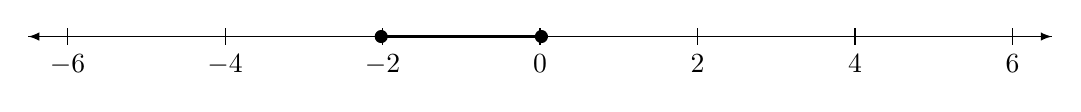
\begin{tikzpicture}
        \draw[latex-] (-6.5,0) -- (6.5,0) ;
        \draw[-latex] (-6.5,0) -- (6.5,0) ;
        \foreach \x in  {-6,-4,-2,0,2,4,6}
        \draw[shift={(\x,0)},color=black] (0pt,3pt) -- (0pt,-3pt);
        \foreach \x in {-6,-4,-2,0,2,4,6}
        \draw[shift={(\x,0)},color=black] (0pt,0pt) -- (0pt,-3pt) node[below]
            {$\x$};
        \draw[*-*] (-2.1,0) -- (0.1,0);
        \draw[very thick    ] (-2.1,0) -- (0.1,0);
    \end{tikzpicture}
    \begin{align*}
        \boxed{(-2, 0)}
    \end{align*}


    \subsection*{301. b}
    \begin{align*}
        -5 \leq x < -3
    \end{align*}
    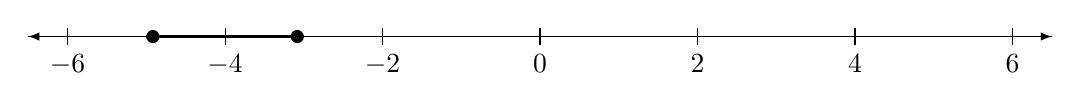
\begin{tikzpicture}
        \draw[latex-] (-6.5,0) -- (6.5,0) ;
        \draw[-latex] (-6.5,0) -- (6.5,0) ;
        \foreach \x in  {-6,-4,-2,0,2,4,6}
        \draw[shift={(\x,0)},color=black] (0pt,3pt) -- (0pt,-3pt);
        \foreach \x in {-6,-4,-2,0,2,4,6}
        \draw[shift={(\x,0)},color=black] (0pt,0pt) -- (0pt,-3pt) node[below]
            {$\x$};
        \draw[*-*] (-5,0) -- (-3,0);
        \draw[very thick    ] (-5,0) -- (-3,0);
    \end{tikzpicture}
    \begin{align*}
        \boxed{[-5, -3)}
    \end{align*}

    \subsection*{301. c}
    \begin{align*}
        0 \leq x \leq 3.5
    \end{align*}
    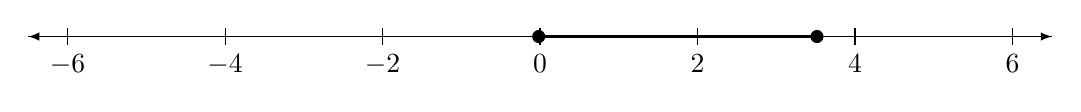
\begin{tikzpicture}
        \draw[latex-] (-6.5,0) -- (6.5,0) ;
        \draw[-latex] (-6.5,0) -- (6.5,0) ;
        \foreach \x in  {-6,-4,-2,0,2,4,6}
        \draw[shift={(\x,0)},color=black] (0pt,3pt) -- (0pt,-3pt);
        \foreach \x in {-6,-4,-2,0,2,4,6}
        \draw[shift={(\x,0)},color=black] (0pt,0pt) -- (0pt,-3pt) node[below]
            {$\x$};
        \draw[*-*] (-0.1,0) -- (3.6,0);
        \draw[very thick    ] (0,0) -- (3.5,0);
    \end{tikzpicture}
    \begin{align*}
        \boxed{[0, 3.5]}
    \end{align*}

    \subsection*{303. a}
    \begin{align*}
        -4 < x < 2
    \end{align*}
    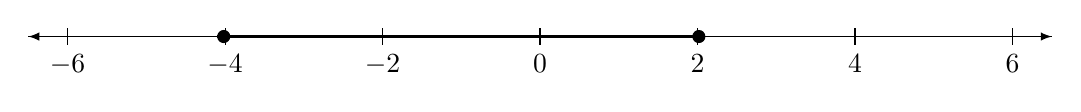
\begin{tikzpicture}
        \draw[latex-] (-6.5,0) -- (6.5,0) ;
        \draw[-latex] (-6.5,0) -- (6.5,0) ;
        \foreach \x in  {-6,-4,-2,0,2,4,6}
        \draw[shift={(\x,0)},color=black] (0pt,3pt) -- (0pt,-3pt);
        \foreach \x in {-6,-4,-2,0,2,4,6}
        \draw[shift={(\x,0)},color=black] (0pt,0pt) -- (0pt,-3pt) node[below]
            {$\x$};
        \draw[*-*] (-4.1,0) -- (2.1,0);
        \draw[very thick    ] (-4.1, 0) -- (2.1,0);
    \end{tikzpicture}
    \begin{align*}
        \boxed{(-4, 2)}
    \end{align*}

    \subsection*{303. b}
    \begin{align*}
        -5 < x \leq -2
    \end{align*}
    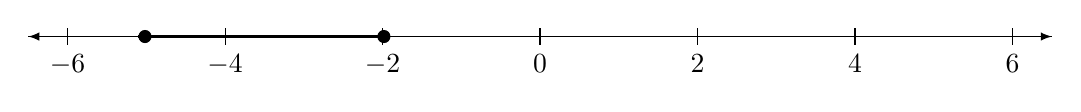
\begin{tikzpicture}
        \draw[latex-] (-6.5,0) -- (6.5,0) ;
        \draw[-latex] (-6.5,0) -- (6.5,0) ;
        \foreach \x in  {-6,-4,-2,0,2,4,6}
        \draw[shift={(\x,0)},color=black] (0pt,3pt) -- (0pt,-3pt);
        \foreach \x in {-6,-4,-2,0,2,4,6}
        \draw[shift={(\x,0)},color=black] (0pt,0pt) -- (0pt,-3pt) node[below]
            {$\x$};
        \draw[*-*] (-5.1,0) -- (-1.9,0);
        \draw[very thick    ] (-5.1, 0) -- (-1.9,0);
    \end{tikzpicture}
    \begin{align*}
        \boxed{(-5, -2]}
    \end{align*}

    \subsection*{303. c}
    \begin{align*}
        -3.75 \leq x \leq 0
    \end{align*}
    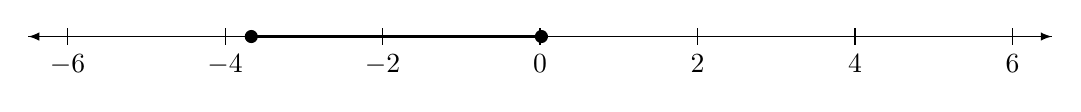
\begin{tikzpicture}
        \draw[latex-] (-6.5,0) -- (6.5,0) ;
        \draw[-latex] (-6.5,0) -- (6.5,0) ;
        \foreach \x in  {-6,-4,-2,0,2,4,6}
        \draw[shift={(\x,0)},color=black] (0pt,3pt) -- (0pt,-3pt);
        \foreach \x in {-6,-4,-2,0,2,4,6}
        \draw[shift={(\x,0)},color=black] (0pt,0pt) -- (0pt,-3pt) node[below]
            {$\x$};
        \draw[*-*] (-3.75,0) -- (0.1,0);
        \draw[very thick    ] (-3.75, 0) -- (0.1,0);
    \end{tikzpicture}
    \begin{align*}
        \boxed{[-3.75, 0]}
    \end{align*}


    \subsection*{305. a}
    \begin{align*}
        & b + \frac{7}{8} \geq \frac{1}{6} \\
        & b \cancel{ + \frac{7}{8}} \geq \frac{1}{6} - \frac{7}{8} \\
        & b \geq \frac{17}{24}
    \end{align*}
    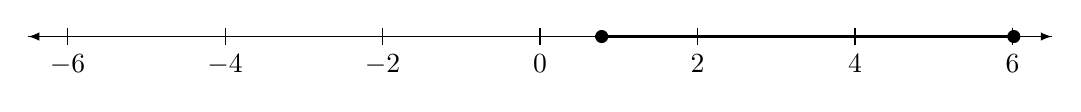
\begin{tikzpicture}
        \draw[latex-] (-6.5,0) -- (6.5,0) ;
        \draw[-latex] (-6.5,0) -- (6.5,0) ;
        \foreach \x in  {-6,-4,-2,0,2,4,6}
        \draw[shift={(\x,0)},color=black] (0pt,3pt) -- (0pt,-3pt);
        \foreach \x in {-6,-4,-2,0,2,4,6}
        \draw[shift={(\x,0)},color=black] (0pt,0pt) -- (0pt,-3pt) node[below]
            {$\x$};
        \draw[*-*] (0.70,0) -- (6.1,0);
        \draw[very thick    ] (0.70, 0) -- (6.1,0);
    \end{tikzpicture}
    \begin{align*}
        \boxed{[\frac{17}{24}, \infty)}
    \end{align*}

    \subsection*{305. b}
    \begin{align*}
        & 6y < 48 \\
        & \frac{6y}{6} < \frac{48}{6} \\
        & y < 8
    \end{align*}
    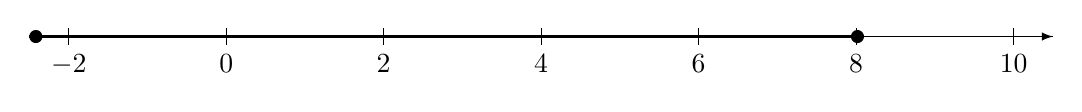
\begin{tikzpicture}
        \draw[latex-] (-2.5,0) -- (10.5,0) ;
        \draw[-latex] (-2.5,0) -- (10.5,0) ;
        \foreach \x in  {-2, 0, 2,4,6,8,10}
        \draw[shift={(\x,0)},color=black] (0pt,3pt) -- (0pt,-3pt);
        \foreach \x in {-2, 0, 2,4,6,8,10}
        \draw[shift={(\x,0)},color=black] (0pt,0pt) -- (0pt,-3pt) node[below]
            {$\x$};
        \draw[*-*] (-2.5,0) -- (8.1,0);
        \draw[very thick    ]  (-2.5,0) -- (8.1,0);
    \end{tikzpicture}
    \begin{align*}
        \boxed{(-\infty, 8)}
    \end{align*}

    \subsection*{305. c}
    \begin{align*}
        & 40 < \frac{5}{8}k \\
        & 8 \times 40 < 8 \times \frac{5}{8}k \\
        & 320 < 5k \\
        & \frac{320}{5} < \frac{5k}{5} \\
        & 64 < k \\
        & k > 64
    \end{align*}
    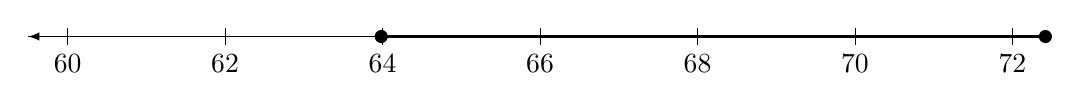
\begin{tikzpicture}
        \draw[latex-] (59.5,0) -- (72.5,0) ;
        \draw[-latex] (59.5,0) -- (72.5,0) ;
        \foreach \x in  {60 , 62, 64, 66, 68, 70, 72}
        \draw[shift={(\x,0)},color=black] (0pt,3pt) -- (0pt,-3pt);
        \foreach \x in  {60 , 62, 64, 66, 68, 70, 72}
        \draw[shift={(\x,0)},color=black] (0pt,0pt) -- (0pt,-3pt) node[below]
            {$\x$};
        \draw[*-*] (63.9,0) -- (72.5,0);
        \draw[very thick    ]  (63.9,0) -- (72.5,0);
    \end{tikzpicture}
    \begin{align*}
        \boxed{(64, \infty)}
    \end{align*}


    \subsection*{307. a}
    \begin{align*}
        & g - \frac{11}{12} < - \frac{5}{18} \\
        & g \cancel{- \frac{11}{12}} < - \frac{5}{18} + \frac{11}{12}\\
        & g < - \frac{10}{36} + \frac{33}{36}\\
        & g < \frac{23}{36}
    \end{align*}
    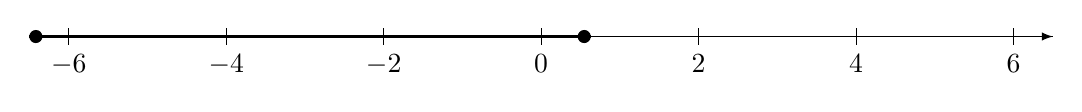
\begin{tikzpicture}
        \draw[latex-] (-6.5,0) -- (6.5,0) ;
        \draw[-latex] (-6.5,0) -- (6.5,0) ;
        \foreach \x in  {-6,-4,-2,0,2,4,6}
        \draw[shift={(\x,0)},color=black] (0pt,3pt) -- (0pt,-3pt);
        \foreach \x in {-6,-4,-2,0,2,4,6}
        \draw[shift={(\x,0)},color=black] (0pt,0pt) -- (0pt,-3pt) node[below]
            {$\x$};
        \draw[*-*] (-6.5,0) -- (0.63,0);
        \draw[very thick    ] (-6.5,0) -- (0.63,0);
    \end{tikzpicture}
    \begin{align*}
        \boxed{(-\infty , \frac{23}{36})}
    \end{align*}


    \subsection*{307. b}
    \begin{align*}
        & 7s < - 28 \\
        & \frac{7s}{7} <  - \frac{28}{7} \\
        & s < - 4
    \end{align*}
    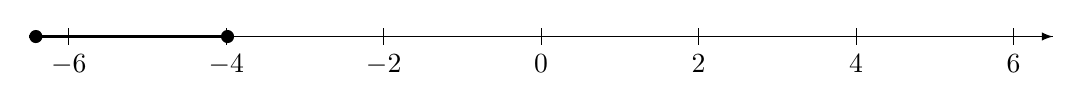
\begin{tikzpicture}
        \draw[latex-] (-6.5,0) -- (6.5,0) ;
        \draw[-latex] (-6.5,0) -- (6.5,0) ;
        \foreach \x in  {-6,-4,-2,0,2,4,6}
        \draw[shift={(\x,0)},color=black] (0pt,3pt) -- (0pt,-3pt);
        \foreach \x in {-6,-4,-2,0,2,4,6}
        \draw[shift={(\x,0)},color=black] (0pt,0pt) -- (0pt,-3pt) node[below]
            {$\x$};
        \draw[*-*] (-6.5,0) -- (-3.9,0);
        \draw[very thick    ] (-6.5,0) -- (-3.9,0);
    \end{tikzpicture}
    \begin{align*}
        \boxed{(-\infty , -4)}
    \end{align*}

    \subsection*{307. c}
    \begin{align*}
        & \frac{9}{4}g \leq 36  \\
        & 4 \times \frac{9}{4}g \leq 4 \times 36  \\
        & 9g \leq 144 \\
        & \frac{9g}{9} \leq \frac{144}{9} \\
        & g \leq 16
    \end{align*}
    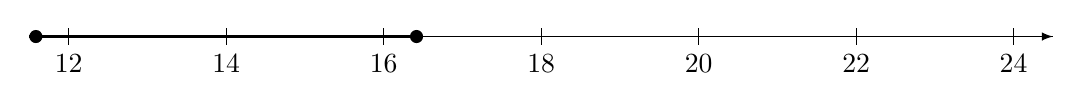
\begin{tikzpicture}
        \draw[latex-] (11.5,0) -- (24.5,0) ;
        \draw[-latex] (11.5,0) -- (24.5,0) ;
        \foreach \x in  {12, 14, 16, 18, 20, 22, 24}
        \draw[shift={(\x,0)},color=black] (0pt,3pt) -- (0pt,-3pt);
        \foreach \x in  {12, 14, 16, 18, 20, 22, 24}
        \draw[shift={(\x,0)},color=black] (0pt,0pt) -- (0pt,-3pt) node[below]
            {$\x$};
        \draw[*-*] (11.5,0) -- (16.5,0);
        \draw[very thick    ] (11.5,0) -- (16.5,0);
    \end{tikzpicture}
    \begin{align*}
        \boxed{(-\infty , 16]}
    \end{align*}


    \subsection*{309. a}
    \begin{align*}
        & -8v \leq 96  \\
        & \frac{-8v}{-8} \leq \frac{96}{-8}  \\
        & v \geq -12
    \end{align*}
    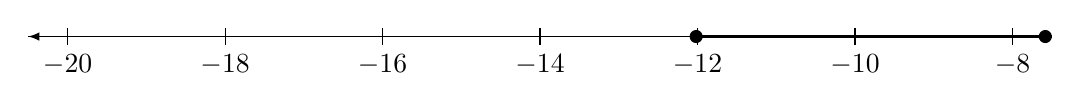
\begin{tikzpicture}
        \draw[latex-] (-20.5,0) -- (-7.5,0) ;
        \draw[-latex] (-20.5,0) -- (-7.5,0) ;
        \foreach \x in  {-20, -18, -16, -14, -12, -10, -8}
        \draw[shift={(\x,0)},color=black] (0pt,3pt) -- (0pt,-3pt);
        \foreach \x in  {-20, -18, -16, -14, -12, -10, -8}
        \draw[shift={(\x,0)},color=black] (0pt,0pt) -- (0pt,-3pt) node[below]
            {$\x$};
        \draw[*-*] (-12.1,0) -- (-7.5,0);
        \draw[very thick    ] (-12.1,0) -- (-7.5,0);
    \end{tikzpicture}
    \begin{align*}
        \boxed{[-12,\infty)}
    \end{align*}


    \subsection*{309. b}
    \begin{align*}
        & \frac{b}{-10} \geq 30  \\
        & -10 \times \frac{b}{-10} \leq -10 \times 30  \\
        & b \leq -300 \\
    \end{align*}
    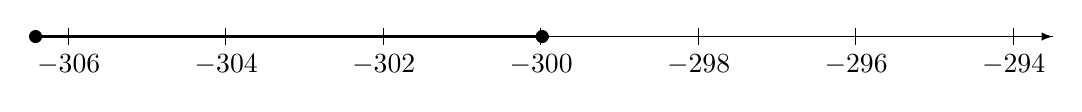
\begin{tikzpicture}
        \draw[latex-] (-306.5,0) -- (-293.5,0) ;
        \draw[-latex] (-306.5,0) -- (-293.5,0) ;
        \foreach \x in  {-306, -304, -302, -300, -298, -296, -294}
        \draw[shift={(\x,0)},color=black] (0pt,3pt) -- (0pt,-3pt);
        \foreach \x in  {-306, -304, -302, -300, -298, -296, -294}
        \draw[shift={(\x,0)},color=black] (0pt,0pt) -- (0pt,-3pt) node[below]
            {$\x$};
        \draw[*-*] (-306.5,0) -- (-299.9,0);
        \draw[very thick    ]  (-306.5,0) -- (-299.9,0);
    \end{tikzpicture}
    \begin{align*}
        \boxed{(-\infty, -300]}
    \end{align*}


    \subsection*{311. a}
    \begin{align*}
        & -7d > 105  \\
        & \frac{-7d}{-7} < \frac{105}{-7}  \\
        & d < -15 \\
    \end{align*}
    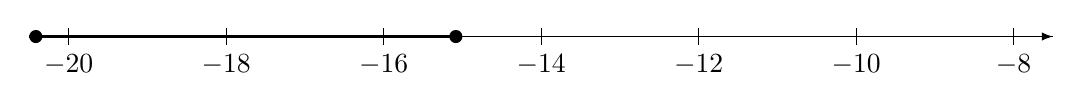
\begin{tikzpicture}
        \draw[latex-] (-20.5,0) -- (-7.5,0) ;
        \draw[-latex] (-20.5,0) -- (-7.5,0) ;
        \foreach \x in  {-20, -18, -16, -14, -12, -10, -8}
        \draw[shift={(\x,0)},color=black] (0pt,3pt) -- (0pt,-3pt);
        \foreach \x in  {-20, -18, -16, -14, -12, -10, -8}
        \draw[shift={(\x,0)},color=black] (0pt,0pt) -- (0pt,-3pt) node[below]
            {$\x$};
        \draw[*-*] (-20.5,0) -- (-15,0);
        \draw[very thick    ]  (-20.5,0) -- (-15,0);
    \end{tikzpicture}
    \begin{align*}
        \boxed{(-\infty, -15)}
    \end{align*}

    \subsection*{311. b}
    \begin{align*}
        & -18 > \frac{q}{-6}  \\
        & -6 \times -18 < -6 \times \frac{q}{-6}  \\
        & 108 < q \\
    \end{align*}
    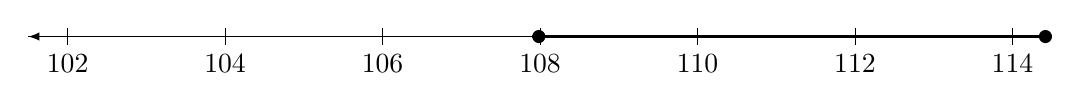
\begin{tikzpicture}
        \draw[latex-] (101.5,0) -- (114.5,0) ;
        \draw[-latex] (101.5,0) -- (114.5,0) ;
        \foreach \x in  {102, 104, 106, 108, 110, 112, 114}
        \draw[shift={(\x,0)},color=black] (0pt,3pt) -- (0pt,-3pt);
        \foreach \x in {102, 104, 106, 108, 110, 112, 114}
        \draw[shift={(\x,0)},color=black] (0pt,0pt) -- (0pt,-3pt) node[below]
            {$\x$};
        \draw[*-*] (107.9,0) -- (114.5,0);
        \draw[very thick    ]   (107.9,0) -- (114.5,0);
    \end{tikzpicture}
    \begin{align*}
        \boxed{(108, \infty)}
    \end{align*}


    \subsection*{313}
    \begin{align*}
        & 5u \leq 8u - 21  \\
        & -8u + 5u \leq \cancel{8u} -21\\
        & -3u \leq -21\\
        & \frac{-3u}{-3} \geq \frac{-21}{-3} \\
        & u \geq 7
    \end{align*}
    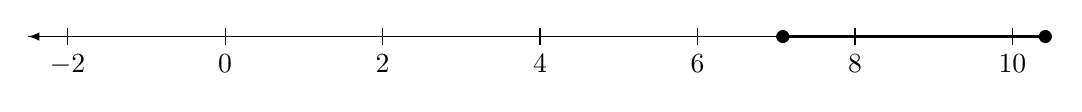
\begin{tikzpicture}
        \draw[latex-] (-2.5,0) -- (10.5,0) ;
        \draw[-latex] (-2.5,0) -- (10.5,0) ;
        \foreach \x in  {-2, 0, 2,4,6,8,10}
        \draw[shift={(\x,0)},color=black] (0pt,3pt) -- (0pt,-3pt);
        \foreach \x in {-2, 0, 2,4,6,8,10}
        \draw[shift={(\x,0)},color=black] (0pt,0pt) -- (0pt,-3pt) node[below]
            {$\x$};
        \draw[*-*] (7,0) -- (10.5,0);
        \draw[very thick    ]  (7,0) -- (10.5,0);
    \end{tikzpicture}
    \begin{align*}
        \boxed{[7, \infty)}
    \end{align*}


    \subsection*{315}
    \begin{align*}
        & 9p > 14p - 18  \\
        & -14p + 9p > \cancel{9p} - 18\\
        & -5p > -18 \\
        & \frac{-5p}{-5} < \frac{-18}{-5}\\
        & p < \frac{18}{5}
    \end{align*}
    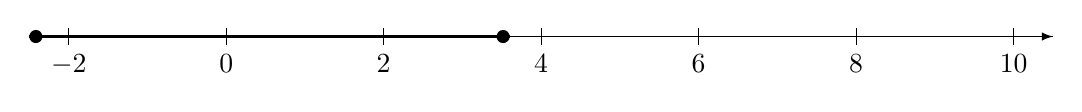
\begin{tikzpicture}
        \draw[latex-] (-2.5,0) -- (10.5,0) ;
        \draw[-latex] (-2.5,0) -- (10.5,0) ;
        \foreach \x in  {-2, 0, 2,4,6,8,10}
        \draw[shift={(\x,0)},color=black] (0pt,3pt) -- (0pt,-3pt);
        \foreach \x in {-2, 0, 2,4,6,8,10}
        \draw[shift={(\x,0)},color=black] (0pt,0pt) -- (0pt,-3pt) node[below]
            {$\x$};
        \draw[*-*] (-2.5,0) -- (3.6,0);
        \draw[very thick    ] (-2.5,0) -- (3.6,0);
    \end{tikzpicture}
    \begin{align*}
        \boxed{(-\infty, \frac{18}{5})}
    \end{align*}


    \subsection*{317}
    \begin{align*}
        & 9y + 5(y + 3) < 4y -35  \\
        & 9y + \tikzmark{MarkA}5(y\tikzmark{MarkB} + 3\tikzmark{MarkC})\DrawBox{black}{black} < 4y -35\\
        & 9y + 5y + 15 < 4y -35\\
        & 14y + 15 < 4y - 35\\
        & -4y + 14y + 15 < \cancel{4y} - 35 \\
        & 10y + 15 < -35 \\
        & 10y \cancel{+ 15} < -35 - 15 \\
        & 10y < -50 \\
        & \frac{10y}{10} < \frac{-50}{10} \\
        & y < - 5
    \end{align*}
    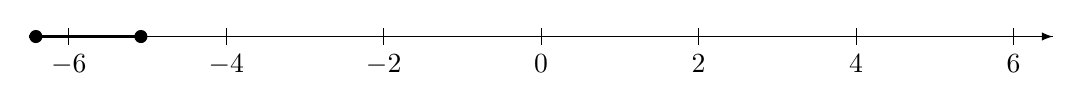
\begin{tikzpicture}
        \draw[latex-] (-6.5,0) -- (6.5,0) ;
        \draw[-latex] (-6.5,0) -- (6.5,0) ;
        \foreach \x in  {-6,-4,-2,0,2,4,6}
        \draw[shift={(\x,0)},color=black] (0pt,3pt) -- (0pt,-3pt);
        \foreach \x in {-6,-4,-2,0,2,4,6}
        \draw[shift={(\x,0)},color=black] (0pt,0pt) -- (0pt,-3pt) node[below]
            {$\x$};
        \draw[*-*] (-6.5,0) -- (-5,0);
        \draw[very thick    ] (-6.5,0) -- (-5,0);
    \end{tikzpicture}
    \begin{align*}
        \boxed{(-\infty, -5)}
    \end{align*}

    \subsection*{319}
    \begin{align*}
        & 4k - (k - 2) \geq 7k -26 \\
        & 4k -\tikzmark{MarkA} (k\tikzmark{MarkB} - 2\tikzmark{MarkC})\DrawBox{black}{black} \geq 7k -26 \\
        & 4k -k -2 \geq 7k - 26 \\
        & 3k - 2 \geq 7k - 26 \\
        & - 7k + 3k - 2 \geq \cancel{7k} - 26 \\
        & -4k - 2 \geq -26 \\
        & -4k \cancel{- 2} \geq -26 - 2 \\
        & -4k \geq -28 \\
        & \frac{-4k}{-4} \leq \frac{-28}{-4} \\
        & k \leq 7
    \end{align*}
    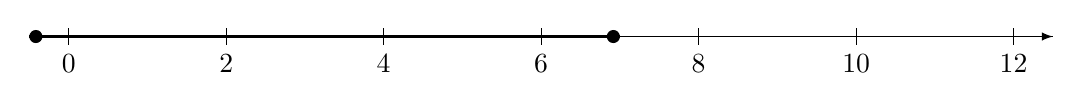
\begin{tikzpicture}
        \draw[latex-] (-0.5,0) -- (12.5,0) ;
        \draw[-latex] (-0.5,0) -- (12.5,0) ;
        \foreach \x in  {0,2,4,6,8,10,12}
        \draw[shift={(\x,0)},color=black] (0pt,3pt) -- (0pt,-3pt);
        \foreach \x in {0,2,4,6,8,10,12}
        \draw[shift={(\x,0)},color=black] (0pt,0pt) -- (0pt,-3pt) node[below]
            {$\x$};
        \draw[*-*] (-0.5,0) -- (7,0);
        \draw[very thick    ] (-0.5,0) -- (7,0);
    \end{tikzpicture}
    \begin{align*}
        \boxed{(-\infty, 7]}
    \end{align*}


    \subsection*{321}
    \begin{align*}
        & 6n - 12(3 - n) \leq 9(n - 4) + 9n \\
        & 6n - \tikzmark{MarkA}12(3\tikzmark{MarkB} - n\tikzmark{MarkC})\DrawBox{black}{black} \leq \tikzmark{MarkA}9(n\tikzmark{MarkB} - 4\tikzmark{MarkC})\DrawBox{black}{black} + 9n \\
        & 6n - 36 + 12n \leq 9n - 36 + 9n \\
        & 18n - 36 \leq 18n - 36\\
        & \cancel{18n} -38 \leq \cancel{18n} -36 \\
        & -36 \leq -36
    \end{align*}
    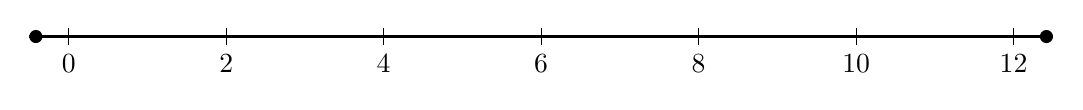
\begin{tikzpicture}
        \draw[latex-] (-0.5,0) -- (12.5,0) ;
        \draw[-latex] (-0.5,0) -- (12.5,0) ;
        \foreach \x in  {0,2,4,6,8,10,12}
        \draw[shift={(\x,0)},color=black] (0pt,3pt) -- (0pt,-3pt);
        \foreach \x in {0,2,4,6,8,10,12}
        \draw[shift={(\x,0)},color=black] (0pt,0pt) -- (0pt,-3pt) node[below]
            {$\x$};
        \draw[*-*] (-0.5,0) -- (12.5,0);
        \draw[very thick    ]  (-0.5,0) -- (12.5,0);
    \end{tikzpicture}
    \begin{align*}
        \boxed{(-\infty, \infty)}
    \end{align*}

    \subsection*{323}
    \begin{align*}
        9u + 5(2u - 5) &\geq 12(u - 1)+ 7u \\
        9u + \tikzmark{MarkA}5(2u\tikzmark{MarkB} - 5\tikzmark{MarkC})\DrawBox{black}{black} &\geq \tikzmark{MarkA}12(u\tikzmark{MarkB} - 1\tikzmark{MarkC})\DrawBox{black}{black}+ 7u \\
        9u + 10u - 25 &\geq 12u - 12 + 7u \\
        \cancel{19u} -25 &\geq \cancel{19u} - 12 \\
        -25 &\geq -12 \\
    \end{align*}
    \begin{tikzpicture}
        \draw[latex-] (-0.5,0) -- (12.5,0) ;
        \draw[-latex] (-0.5,0) -- (12.5,0) ;
        \foreach \x in  {0,2,4,6,8,10,12}
        \draw[shift={(\x,0)},color=black] (0pt,3pt) -- (0pt,-3pt);
        \foreach \x in {0,2,4,6,8,10,12}
        \draw[shift={(\x,0)},color=black] (0pt,0pt) -- (0pt,-3pt) node[below]
            {$\x$};
    \end{tikzpicture}
    \begin{align*}
        \boxed{No solution}
    \end{align*}

    \subsection*{325}
    \begin{align*}
        \frac{4}{5}h - \frac{2}{3}(h - 9) &\geq\frac{1}{5}( 2h+ 90) \\
        \frac{4}{5}h - \tikzmark{MarkA}\frac{2}{3}(h\tikzmark{MarkB} - 9\tikzmark{MarkC})\DrawBox{black}{black} &\geq\tikzmark{MarkA}\frac{1}{5}( 2h\tikzmark{MarkB}+ 90\tikzmark{MarkC})\DrawBox{black}{black}\\
        \frac{4}{5}h - \frac{2}{3}h + 6 & \geq \frac{2}{5}h +18\\
        - \frac{2}{5}h + \frac{4}{5}h - \frac{2}{3}h + 6 & \geq \cancel{\frac{2}{5}h} +18 \\
        \frac{2}{5}h - \frac{2}{3}h + 6 &\geq 18 \\
        \frac{2}{5}h - \frac{2}{3}h \cancel{+ 6} &\geq 18 - 6 \\
        \frac{2}{5}h - \frac{2}{3}h &\geq 12 \\
        15 (\frac{2}{5}h - \frac{2}{3}h) &\geq 15 \times 12 \\
        6h  - 10h & \geq 180 \\
        -4h & \geq 180 \\
        \frac{-4h}{-4} &\leq \frac{180}{-4} \\
        h &\leq -45
    \end{align*}
    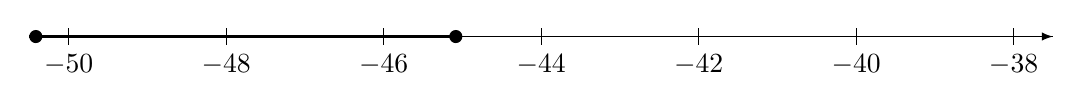
\begin{tikzpicture}
        \draw[latex-] (-50.5,0) -- (-37.5,0) ;
        \draw[-latex]  (-50.5,0) -- (-37.5,0) ;
        \foreach \x in  {-50, -48, -46, -44, -42, -40, -38}
        \draw[shift={(\x,0)},color=black] (0pt,3pt) -- (0pt,-3pt);
        \foreach \x in {-50, -48, -46, -44, -42, -40, -38}
        \draw[shift={(\x,0)},color=black] (0pt,0pt) -- (0pt,-3pt) node[below]
            {$\x$};
        \draw[*-*] (-50.5,0) -- (-45,0);
        \draw[very thick    ]  (-50.5,0) -- (-45,0);
    \end{tikzpicture}
    \begin{align*}
        \boxed{(\infty,-45]}
    \end{align*}

    \subsection*{327}
    \begin{align*}
        12v + 3(4v-1) &\leq 19(v-2) + 5v\\
        12v +\tikzmark{MarkA}3(4v\tikzmark{MarkB} - 1\tikzmark{MarkC})\DrawBox{black}{black} &\leq\tikzmark{MarkA}19( v\tikzmark{MarkB}-2\tikzmark{MarkC})\DrawBox{black}{black}+5v\\
        12v + 12v - 3 &\leq 19v - 38 + 5v \\
        24v - 3 & \leq 24v - 38 \\
        \cancel{24v} - 3 & \leq \cancel{24v} - 38 \\
        - 3 & \leq  - 38 \\
    \end{align*}
    \begin{tikzpicture}
        \draw[latex-] (-0.5,0) -- (12.5,0) ;
        \draw[-latex] (-0.5,0) -- (12.5,0) ;
        \foreach \x in  {0,2,4,6,8,10,12}
        \draw[shift={(\x,0)},color=black] (0pt,3pt) -- (0pt,-3pt);
        \foreach \x in {0,2,4,6,8,10,12}
        \draw[shift={(\x,0)},color=black] (0pt,0pt) -- (0pt,-3pt) node[below]
            {$\x$};
    \end{tikzpicture}
    \begin{align*}
        \boxed{No solution}
    \end{align*}

    \subsection*{329}
    \begin{align*}
        35k &\geq -77\\
        \frac{35k}{35} &\geq \frac{-77}{35}\\
        k &\geq -\frac{77 \div 7}{35 \div 7} \\
        k & \geq -\frac{11}{5}
    \end{align*}
    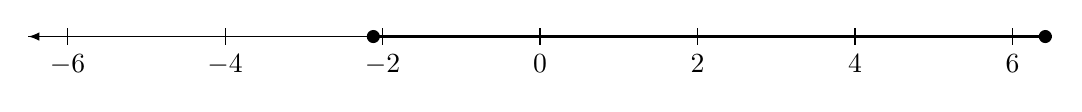
\begin{tikzpicture}
        \draw[latex-] (-6.5,0) -- (6.5,0) ;
        \draw[-latex] (-6.5,0) -- (6.5,0) ;
        \foreach \x in  {-6,-4,-2,0,2,4,6}
        \draw[shift={(\x,0)},color=black] (0pt,3pt) -- (0pt,-3pt);
        \foreach \x in {-6,-4,-2,0,2,4,6}
        \draw[shift={(\x,0)},color=black] (0pt,0pt) -- (0pt,-3pt) node[below]
            {$\x$};
        \draw[*-*] (-2.2,0) -- (6.5,0);
        \draw[very thick    ] (-2.2,0) -- (6.5,0);
    \end{tikzpicture}
    \begin{align*}
        \boxed{[-\frac{11}{5},\infty)}
    \end{align*}


    \subsection*{331}
    \begin{align*}
        18q -4(10 - 3q) &< 5(6q - 8) \\
        18q -4\tikzmark{MarkA}(10\tikzmark{MarkB} - 3q\tikzmark{MarkC})\DrawBox{black}{black} &< \tikzmark{MarkA}5(6q\tikzmark{MarkB} -8\tikzmark{MarkC})\DrawBox{black}{black}\\
        18q -40 + 12q &< 30q - 40 \\
        30q -40  &< 30q - 40 \\
        \cancel{30q} -40 &< \cancel{30q} -40 \\
        -40 &< -40
    \end{align*}
    \begin{tikzpicture}
        \draw[latex-] (-6.5,0) -- (6.5,0) ;
        \draw[-latex] (-6.5,0) -- (6.5,0) ;
        \foreach \x in  {-6,-4,-2,0,2,4,6}
        \draw[shift={(\x,0)},color=black] (0pt,3pt) -- (0pt,-3pt);
        \foreach \x in {-6,-4,-2,0,2,4,6}
        \draw[shift={(\x,0)},color=black] (0pt,0pt) -- (0pt,-3pt) node[below]
            {$\x$};
    \end{tikzpicture}
    \begin{align*}
        \boxed{No Solution}
    \end{align*}


    \subsection*{335}
    \begin{align*}
        d+ 29 &> 61 \\
        d \cancel{+29} &> -61 - 29 \\
        d &> -90 \\
    \end{align*}
    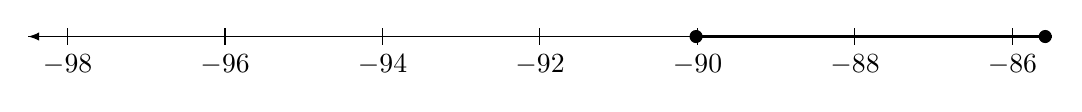
\begin{tikzpicture}
        \draw[latex-] (-98.5,0) -- (-85.5,0) ;
        \draw[-latex] (-98.5,0) -- (-85.5,0) ;
        \foreach \x in  {-98,-96,-94,-92,-90,-88,-86}
        \draw[shift={(\x,0)},color=black] (0pt,3pt) -- (0pt,-3pt);
        \foreach \x in {-98,-96,-94,-92,-90,-88,-86}
        \draw[shift={(\x,0)},color=black] (0pt,0pt) -- (0pt,-3pt) node[below]
            {$\x$};
        \draw[*-*] (-90.1,0) -- (-85.5,0);
        \draw[very thick    ] (-90.1,0) -- (-85.5,0);
    \end{tikzpicture}
    \begin{align*}
        \boxed{(-90, \infty)}
    \end{align*}

    \section*{2.6 377 to 425 odd}
    \subsection*{377}
    \begin{align*}
        x \leq 4 \hspace{.2cm} an&d \hspace{.2cm} x > -2 \\
        -2 < &x \leq 4
    \end{align*}
    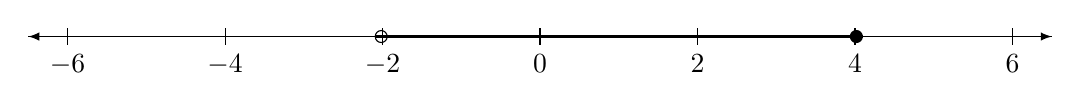
\begin{tikzpicture}
        \draw[latex-] (-6.5,0) -- (6.5,0) ;
        \draw[-latex] (-6.5,0) -- (6.5,0) ;
        \foreach \x in  {-6,-4,-2,0,2,4,6}
        \draw[shift={(\x,0)},color=black] (0pt,3pt) -- (0pt,-3pt);
        \foreach \x in {-6,-4,-2,0,2,4,6}
        \draw[shift={(\x,0)},color=black] (0pt,0pt) -- (0pt,-3pt) node[below]
            {$\x$};
        \draw[o-*] (-2.1,0) -- (4.1,0);
        \draw[very thick    ] (-2.1,0) -- (4.1,0);
    \end{tikzpicture}
    \begin{align*}
        \boxed{(-2,4]}
    \end{align*}


    \subsection*{379}
    \begin{align*}
        x > -6 \hspace{.2cm} an&d \hspace{.2cm} x < -3 \\
        -6 < x& < -3
    \end{align*}
    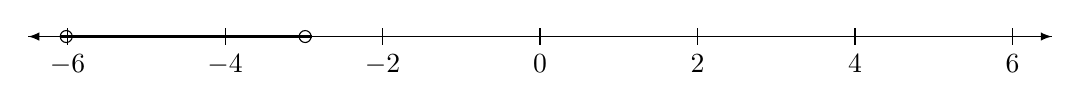
\begin{tikzpicture}
        \draw[latex-] (-6.5,0) -- (6.5,0) ;
        \draw[-latex] (-6.5,0) -- (6.5,0) ;
        \foreach \x in  {-6,-4,-2,0,2,4,6}
        \draw[shift={(\x,0)},color=black] (0pt,3pt) -- (0pt,-3pt);
        \foreach \x in {-6,-4,-2,0,2,4,6}
        \draw[shift={(\x,0)},color=black] (0pt,0pt) -- (0pt,-3pt) node[below]
            {$\x$};
        \draw[o-o] (-6.1,0) -- (-2.9,0);
        \draw[very thick    ](-6.1,0) -- (-2.9,0);
    \end{tikzpicture}
    \begin{align*}
        \boxed{(-6,-3)}
    \end{align*}

    \subsection*{381}
    \begin{align*}
        4x -1 &< 7 \hspace{2cm} and &2x + 8 &\geq 4 \\
        4x \cancel{-1} &< 7 + 1 &2x \cancel{+ 8} &\geq 4 - 8 \\
        4x &< 8  &2x &\geq -4 \\
        \frac{4x}{4} &< \frac{8}{4}  &\frac{2x}{2} &\geq \frac{-4}{2} \\
        x &< 2  &x &\geq -2 \\
        &\hspace{2cm} -2 \leq x < 2
    \end{align*}
    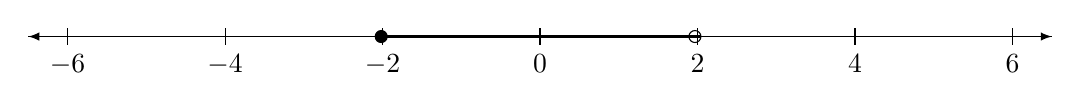
\begin{tikzpicture}
        \draw[latex-] (-6.5,0) -- (6.5,0) ;
        \draw[-latex] (-6.5,0) -- (6.5,0) ;
        \foreach \x in  {-6,-4,-2,0,2,4,6}
        \draw[shift={(\x,0)},color=black] (0pt,3pt) -- (0pt,-3pt);
        \foreach \x in {-6,-4,-2,0,2,4,6}
        \draw[shift={(\x,0)},color=black] (0pt,0pt) -- (0pt,-3pt) node[below]
            {$\x$};
        \draw[*-o] (-2.1,0) -- (2.05,0);
        \draw[very thick    ](-2.1,0) -- (2.05,0);
    \end{tikzpicture}
    \begin{align*}
        \boxed{[-2, 2)}
    \end{align*}

    \subsection*{383}
    \begin{align*}
        4x -2 &\leq 4 \hspace{2cm} and &7x - 1 &> -8 \\
        4x \cancel{-2} &\leq 4 + 2 &7x \cancel{- 1} &> - 8 + 1 \\
        4x &\leq 6   &7x &> -7 \\
        \frac{4x}{4} &\leq \frac{6}{4}  &\frac{7x}{7} &> \frac{-7}{7} \\
        x &\leq \frac{3}{2}  &x &> -1 \\
        &\hspace{2cm} -1 < x \leq \frac{2}{3}
    \end{align*}
    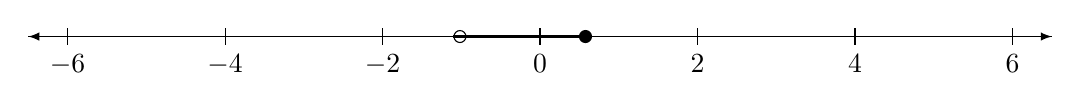
\begin{tikzpicture}
        \draw[latex-] (-6.5,0) -- (6.5,0) ;
        \draw[-latex] (-6.5,0) -- (6.5,0) ;
        \foreach \x in  {-6,-4,-2,0,2,4,6}
        \draw[shift={(\x,0)},color=black] (0pt,3pt) -- (0pt,-3pt);
        \foreach \x in {-6,-4,-2,0,2,4,6}
        \draw[shift={(\x,0)},color=black] (0pt,0pt) -- (0pt,-3pt) node[below]
            {$\x$};
        \draw[o-*] (-1.1,0) -- (.66,0);
        \draw[very thick    ](-1.1,0) -- (.66,0);
    \end{tikzpicture}
    \begin{align*}
        \boxed{(-1, \frac{3}{2}]}
    \end{align*}


    \subsection*{385}
    \begin{align*}
        7x -8 &< 6 \hspace{2cm} and &5x + 7 &> -3 \\
        7x \cancel{-8} &< 6 + 8 &5x \cancel{+ 7} &> -3 -7 \\
        7x &< 14   &5x &> -10 \\
        \frac{7x}{7} &< \frac{14}{7}  &\frac{5x}{5} &> \frac{-10}{5} \\
        x &< 2  &x &> -2 \\
        &\hspace{2cm} -2 < x < 2
    \end{align*}
    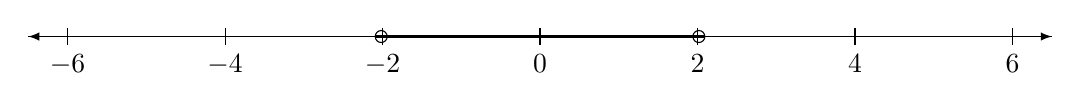
\begin{tikzpicture}
        \draw[latex-] (-6.5,0) -- (6.5,0) ;
        \draw[-latex] (-6.5,0) -- (6.5,0) ;
        \foreach \x in  {-6,-4,-2,0,2,4,6}
        \draw[shift={(\x,0)},color=black] (0pt,3pt) -- (0pt,-3pt);
        \foreach \x in {-6,-4,-2,0,2,4,6}
        \draw[shift={(\x,0)},color=black] (0pt,0pt) -- (0pt,-3pt) node[below]
            {$\x$};
        \draw[o-o] (-2.1,0) -- (2.1,0);
        \draw[very thick    ](-2.1,0) -- (2.1,0);
    \end{tikzpicture}
    \begin{align*}
        \boxed{(-2,-2)}
    \end{align*}


    \subsection*{387}
    \begin{align*}
        5(3x-2) &\leq 5 \hspace{2cm} and &3(x + 3) &< 3 \\
        15x - 10 &\leq 5 &3x + 9 &< 3 \\
        15x \cancel{-10} &\leq 5 + 10 &3x \cancel{+ 9} &< 3  - 9 \\
        15x &\leq 15   &3x &< -6 \\
        \frac{15x}{15} &\leq \frac{15}{15}  &\frac{3x}{3} &< \frac{-6}{3} \\
        x &\leq 1  &x &< -2 \\
        &\hspace{2.5cm} x < 2
    \end{align*}
    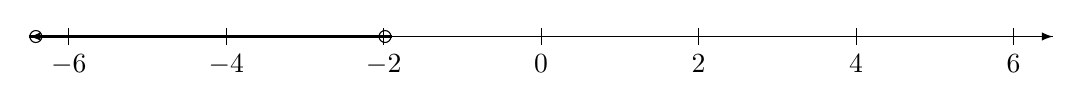
\begin{tikzpicture}
        \draw[latex-] (-6.5,0) -- (6.5,0) ;
        \draw[-latex] (-6.5,0) -- (6.5,0) ;
        \foreach \x in  {-6,-4,-2,0,2,4,6}
        \draw[shift={(\x,0)},color=black] (0pt,3pt) -- (0pt,-3pt);
        \foreach \x in {-6,-4,-2,0,2,4,6}
        \draw[shift={(\x,0)},color=black] (0pt,0pt) -- (0pt,-3pt) node[below]
            {$\x$};
        \draw[o-o] (-6.5,0) -- (-1.9,0);
        \draw[very thick    ](-6.5,0) -- (-1.9,0);
    \end{tikzpicture}
    \begin{align*}
        \boxed{(-\infty,-2)}
    \end{align*}


    \subsection*{389}
    \begin{align*}
        -3(x+4) &< 0 \hspace{2cm} and &-1(3x - 1) &\leq 7 \\
        -3x - 12 &< 0 &-3x + 1 &\leq 7 \\
        -3x \cancel{-12} &< 0 + 12 &-3x \cancel{+ 1} &\leq 7  - 1 \\
        -3x &< 12   &-3x &\leq 6 \\
        \frac{-3x}{-3} &< \frac{12}{-3}  &\frac{-3x}{-3} &\leq \frac{6}{-3} \\
        x &> -4  &x &\geq -2 \\
        &\hspace{2.5cm} -2 \leq x
    \end{align*}
    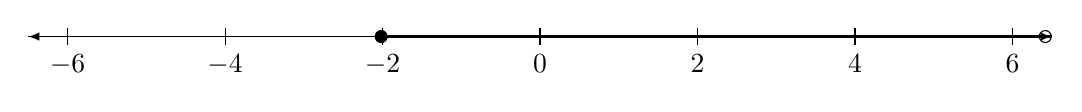
\begin{tikzpicture}
        \draw[latex-] (-6.5,0) -- (6.5,0) ;
        \draw[-latex] (-6.5,0) -- (6.5,0) ;
        \foreach \x in  {-6,-4,-2,0,2,4,6}
        \draw[shift={(\x,0)},color=black] (0pt,3pt) -- (0pt,-3pt);
        \foreach \x in {-6,-4,-2,0,2,4,6}
        \draw[shift={(\x,0)},color=black] (0pt,0pt) -- (0pt,-3pt) node[below]
            {$\x$};
        \draw[*-o] (-2.1,0) -- (6.5,0);
        \draw[very thick    ](-2.1,0) -- (6.5,0);
    \end{tikzpicture}
    \begin{align*}
        \boxed{[-2,\infty)}
    \end{align*}


    \subsection*{391}
    \begin{align*}
        \frac{3}{4}(x-8) &\leq 3 \hspace{2cm} and &\frac{1}{5}(x - 5) &\leq 3 \\
        \frac{3}{4}x -6 &\leq 3 &\frac{1}{5}x - 1 &\leq 3 \\
        \frac{3}{4}x \cancel{-6} &\leq 3 + 6 &\frac{1}{5}x \cancel{- 1} &\leq 3  + 1 \\
        \frac{3}{4}x &\leq 9   &\frac{1}{5}x &\leq 4 \\
        4 \times \frac{3}{4}x &\leq 4 \times 9   &5 \times \frac{1}{5}x &\leq 5 \times 4 \\
        3x &\leq 36   &x &\leq 20 \\
        \frac{3x}{3} &\leq \frac{36}{3}  &x &\leq 20 \\
        x &\leq 12  &x &\leq 20 \\
        &\hspace{2.5cm} x \leq 12
    \end{align*}
    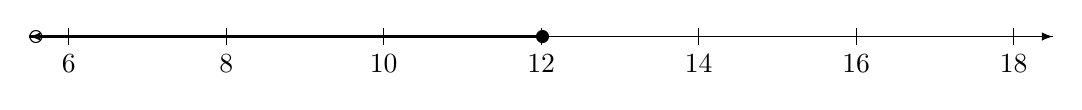
\begin{tikzpicture}
        \draw[latex-] (5.5,0) -- (18.5,0) ;
        \draw[-latex] (5.5,0) -- (18.5,0) ;
        \foreach \x in  {6, 8, 10, 12, 14, 16, 18}
        \draw[shift={(\x,0)},color=black] (0pt,3pt) -- (0pt,-3pt);
        \foreach \x in  {6, 8, 10, 12, 14, 16, 18}
        \draw[shift={(\x,0)},color=black] (0pt,0pt) -- (0pt,-3pt) node[below]
            {$\x$};
        \draw[o-*] (5.5,0) -- (12.1,0);
        \draw[very thick    ](5.5,0) -- (12.1,0);
    \end{tikzpicture}
    \begin{align*}
        \boxed{(-\infty,12]}
    \end{align*}


    \subsection*{393}
    \begin{align*}
        \frac{3}{4}(x-5) &\geq -2 \hspace{2cm} and &-3(x + 1) &\geq 6 \\
        4 \times \frac{3}{4}(x-5) &\geq 4 \times -2  &-3x \cancel{- 3} &\geq 6 + 3 \\
        3(x-5) &\geq -8  &-3x  &\geq 9 \\
        3x-15 &\geq -8  &\frac{-3x}{-3}  &\leq \frac{9}{-3} \\
        3x\cancel{-15} &\geq -8 + 15  &x  &\leq -3\\
        3x &\geq 7  \\
        \frac{3x}{3} &\geq \frac{7}{3}  \\
        x &\geq \frac{7}{3} \\
        x &\geq \frac{7}{3} \hspace{2cm} and &x  &\leq -3
    \end{align*}
    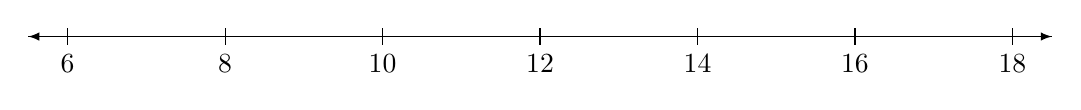
\begin{tikzpicture}
        \draw[latex-] (5.5,0) -- (18.5,0) ;
        \draw[-latex] (5.5,0) -- (18.5,0) ;
        \foreach \x in  {6, 8, 10, 12, 14, 16, 18}
        \draw[shift={(\x,0)},color=black] (0pt,3pt) -- (0pt,-3pt);
        \foreach \x in  {6, 8, 10, 12, 14, 16, 18}
        \draw[shift={(\x,0)},color=black] (0pt,0pt) -- (0pt,-3pt) node[below]
            {$\x$};
    \end{tikzpicture}
    \begin{align*}
        \boxed{No solution}
    \end{align*}

    \subsection*{395}
    \begin{align*}
        \frac{1}{2}(x-6)+2 &< -5 \hspace{2cm} and &4 - \frac{2}{3}x &< 6 \\
        2 (\frac{1}{2}(x-6)+2) &< 2 \times -5 &3(4 - \frac{2}{3}x) &< 3 \times 6\\
        x-6 +4 &< -10 &12 - 2x &< 9\\
        x-2 &< -10  &\cancel{12} - 2x &< 9 -12 \\
        x\cancel{-2} &< -10 + 2  &- 2x &< -3 \\
        x &< -8 &\frac{-2x}{-2} &> \frac{-3}{-2}  \\
        &&x &> \frac{3}{2}  \\
        x &< -8 \hspace{2cm} and &x &> \frac{3}{2}
    \end{align*}
    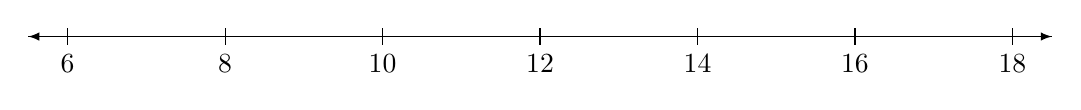
\begin{tikzpicture}
        \draw[latex-] (5.5,0) -- (18.5,0) ;
        \draw[-latex] (5.5,0) -- (18.5,0) ;
        \foreach \x in  {6, 8, 10, 12, 14, 16, 18}
        \draw[shift={(\x,0)},color=black] (0pt,3pt) -- (0pt,-3pt);
        \foreach \x in  {6, 8, 10, 12, 14, 16, 18}
        \draw[shift={(\x,0)},color=black] (0pt,0pt) -- (0pt,-3pt) node[below]
            {$\x$};
    \end{tikzpicture}
    \begin{align*}
        \boxed{No solution}
    \end{align*}


    \subsection*{397}
    \begin{align*}
       -3 &< 2x -5 \leq 1 \\
       -3 + 5 &< 2x \cancel{-5} \leq 1 + 5 \\
       2 &< 2x  \leq 6 \\
       \frac{2}{2} &< \frac{2x}{2}  \leq \frac{6}{2} \\
       1 &< x  \leq 3 \\
    \end{align*}
    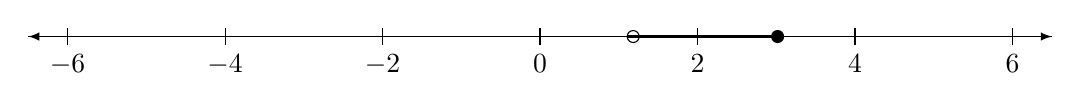
\begin{tikzpicture}
        \draw[latex-] (-6.5,0) -- (6.5,0) ;
        \draw[-latex] (-6.5,0) -- (6.5,0) ;
        \foreach \x in  {-6,-4,-2,0,2,4,6}
        \draw[shift={(\x,0)},color=black] (0pt,3pt) -- (0pt,-3pt);
        \foreach \x in {-6,-4,-2,0,2,4,6}
        \draw[shift={(\x,0)},color=black] (0pt,0pt) -- (0pt,-3pt) node[below]
            {$\x$};
        \draw[o-*] (1.1,0) -- (3.1,0);
        \draw[very thick    ] (1.1,0) -- (3.1,0);
    \end{tikzpicture}
    \begin{align*}
        \boxed{(1, 3]}
    \end{align*}

    \subsection*{399}
    \begin{align*}
        -1 &< 3x +2 < 8 \\
        -1 - 2 &< 3x \cancel{+2} < 8 - 2 \\
        -3 &< 3x  < 6 \\
        \frac{-3}{3} &< \frac{3x}{3} < \frac{6}{3} \\
        -1 &< x  < 2 \\
    \end{align*}
    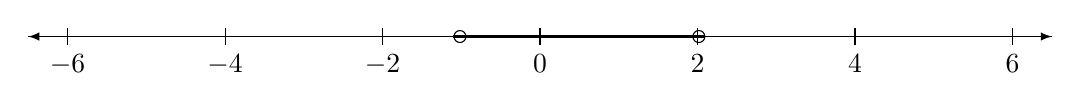
\begin{tikzpicture}
        \draw[latex-] (-6.5,0) -- (6.5,0) ;
        \draw[-latex] (-6.5,0) -- (6.5,0) ;
        \foreach \x in  {-6,-4,-2,0,2,4,6}
        \draw[shift={(\x,0)},color=black] (0pt,3pt) -- (0pt,-3pt);
        \foreach \x in {-6,-4,-2,0,2,4,6}
        \draw[shift={(\x,0)},color=black] (0pt,0pt) -- (0pt,-3pt) node[below]
            {$\x$};
        \draw[o-o] (-1.1,0) -- (2.1,0);
        \draw[very thick    ] (-1.1,0) -- (2.1,0);
    \end{tikzpicture}
    \begin{align*}
        \boxed{(-1, 2)}
    \end{align*}

    \subsection*{401}
    \begin{align*}
        -6 &\leq 4x -2 < -2 \\
        2 -6 &\leq 4x \cancel{-2} < - 2 + 2 \\
        -4 &\leq 4x < 0 \\
        \frac{-4}{4} &\leq \frac{4x}{4} < \frac{0}{4} \\
        -1 &\leq x < 0 \\
    \end{align*}
    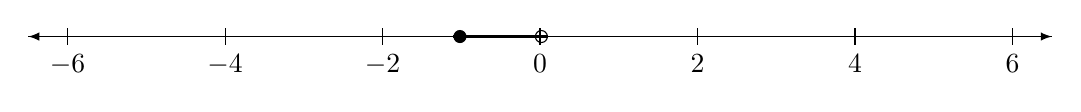
\begin{tikzpicture}
        \draw[latex-] (-6.5,0) -- (6.5,0) ;
        \draw[-latex] (-6.5,0) -- (6.5,0) ;
        \foreach \x in  {-6,-4,-2,0,2,4,6}
        \draw[shift={(\x,0)},color=black] (0pt,3pt) -- (0pt,-3pt);
        \foreach \x in {-6,-4,-2,0,2,4,6}
        \draw[shift={(\x,0)},color=black] (0pt,0pt) -- (0pt,-3pt) node[below]
            {$\x$};
        \draw[*-o] (-1.1,0) -- (0.1,0);
        \draw[very thick    ] (-1.1,0) -- (0.1,0);
    \end{tikzpicture}
    \begin{align*}
        \boxed{[-1, 0)}
    \end{align*}

    \subsection*{403}
    \begin{align*}
        x &\leq -4 \hspace{2cm} or &x  &> -3 \\
    \end{align*}
    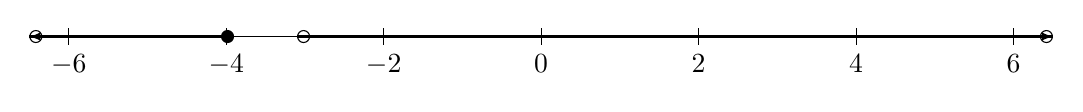
\begin{tikzpicture}
        \draw[latex-] (-6.5,0) -- (6.5,0) ;
        \draw[-latex] (-6.5,0) -- (6.5,0) ;
        \foreach \x in  {-6,-4,-2,0,2,4,6}
        \draw[shift={(\x,0)},color=black] (0pt,3pt) -- (0pt,-3pt);
        \foreach \x in  {-6,-4,-2,0,2,4,6}
        \draw[shift={(\x,0)},color=black] (0pt,0pt) -- (0pt,-3pt) node[below]
            {$\x$};
        \draw[o-*] (-6.5,0) -- (-3.9,0);
        \draw[very thick    ] (-6.5,0) -- (-3.9,0);
        \draw[o-o] (-3.1,0) -- (6.5,0);
        \draw[very thick    ] (-3.1,0) -- (6.5,0);
    \end{tikzpicture}
    \begin{align*}
        \boxed{(-\infty, -4]\cup(-3, \infty)}
    \end{align*}

    \subsection*{405}
    \begin{align*}
        x &< 0 \hspace{2cm} or &x  &\geq 4 \\
    \end{align*}
    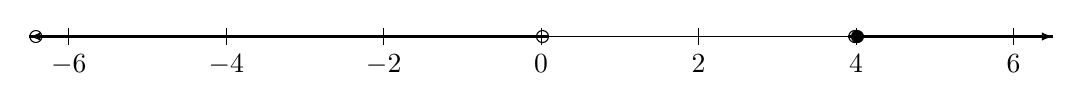
\begin{tikzpicture}
        \draw[latex-] (-6.5,0) -- (6.5,0) ;
        \draw[-latex] (-6.5,0) -- (6.5,0) ;
        \foreach \x in  {-6,-4,-2,0,2,4,6}
        \draw[shift={(\x,0)},color=black] (0pt,3pt) -- (0pt,-3pt);
        \foreach \x in  {-6,-4,-2,0,2,4,6}
        \draw[shift={(\x,0)},color=black] (0pt,0pt) -- (0pt,-3pt) node[below]
            {$\x$};
        \draw[o-o] (-6.5,0) -- (0.1,0);
        \draw[very thick    ] (-6.5,0) -- (0.1,0);
        \draw[*-o] (4.1,0) -- (3.9,0);
        \draw[very thick    ] (3.9,0) -- (6.5,0);
    \end{tikzpicture}
    \begin{align*}
        \boxed{(-\infty, 0)\cup[4, \infty)}
    \end{align*}

    \subsection*{407}
    \begin{align*}
        4 - 3x &\leq -2 \hspace{2cm} or &2x - 1  &\leq -5 \\
        \cancel{4} - 3x &\leq -2 -4  &2x \cancel{- 1}  &\leq -5 + 1 \\
        - 3x &\leq -6  &2x  &\leq -4 \\
        \frac{- 3x}{-3} &\geq \frac{-6}{-3}  &\frac{2x}{2}  &\leq \frac{-4}{2} \\
        x &\geq 2 &x &\leq -2 \\
    \end{align*}
    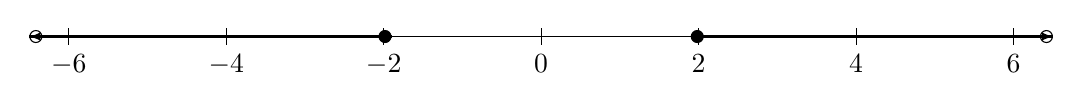
\begin{tikzpicture}
        \draw[latex-] (-6.5,0) -- (6.5,0) ;
        \draw[-latex] (-6.5,0) -- (6.5,0) ;
        \foreach \x in  {-6,-4,-2,0,2,4,6}
        \draw[shift={(\x,0)},color=black] (0pt,3pt) -- (0pt,-3pt);
        \foreach \x in  {-6,-4,-2,0,2,4,6}
        \draw[shift={(\x,0)},color=black] (0pt,0pt) -- (0pt,-3pt) node[below]
            {$\x$};
        \draw[*-o] (1.9,0) -- (6.5,0);
        \draw[very thick    ] (1.9,0) -- (6.5,0);
        \draw[o-*] (-6.5,0) -- (-1.9,0);
        \draw[very thick    ] (-6.5,0) -- (-1.9,0);
    \end{tikzpicture}
    \begin{align*}
        \boxed{(-\infty, -2]\cup[2, \infty)}
    \end{align*}

    \subsection*{409}
    \begin{align*}
        3(2x - 3) &< -5 \hspace{2cm} or &4x - 1  &> 3 \\
        6x - 9 &< -5 &4x \cancel{-1} &> 3 + 1\\
        6x \cancel{-9} &< -5 + 9 &4x &> 4\\
        6x &< 4 &\frac{4x}{4} &> \frac{4}{4} \\
        \frac{6x}{6} &< \frac{4}{6} &x &> 1 \\
        x &< \frac{2}{3} &x &> 1 \\
    \end{align*}
    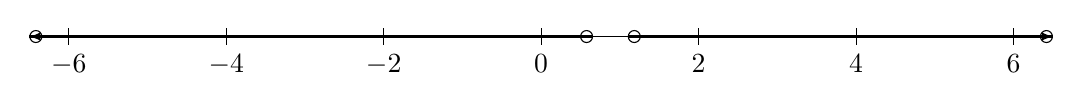
\begin{tikzpicture}
        \draw[latex-] (-6.5,0) -- (6.5,0) ;
        \draw[-latex] (-6.5,0) -- (6.5,0) ;
        \foreach \x in  {-6,-4,-2,0,2,4,6}
        \draw[shift={(\x,0)},color=black] (0pt,3pt) -- (0pt,-3pt);
        \foreach \x in  {-6,-4,-2,0,2,4,6}
        \draw[shift={(\x,0)},color=black] (0pt,0pt) -- (0pt,-3pt) node[below]
            {$\x$};
        \draw[o-o] (-6.5,0) -- (0.66,0);
        \draw[very thick    ] (-6.5,0) -- (0.66,0);
        \draw[o-o] (1.1,0) -- (6.5,0);
        \draw[very thick    ] (1.1,0) -- (6.5,0);
    \end{tikzpicture}
    \begin{align*}
        \boxed{(-\infty, \frac{2}{3})\cup(1, \infty)}
    \end{align*}


    \subsection*{411}
    \begin{align*}
        \frac{2}{3}x - 3 &> 5 \hspace{2cm} or &3(5 - x)  &> 6 \\
        \frac{2}{3}x \cancel{- 3} &> 5 + 3 &15 - 3x  &> 6 \\
        \frac{2}{3}x  &> 8 &\cancel{15} - 3x  &> 6 -15 \\
        3 \times \frac{2}{3}x  &> 3 \times 8 &- 3x  &> -9 \\
        2x &> 24 &\frac{-3x}{3} &< \frac{-9}{-3} \\
        \frac{2x}{2} &> \frac{24}{2} &x &< 3 \\
        x &> 12 &x &< 3 \\
    \end{align*}
    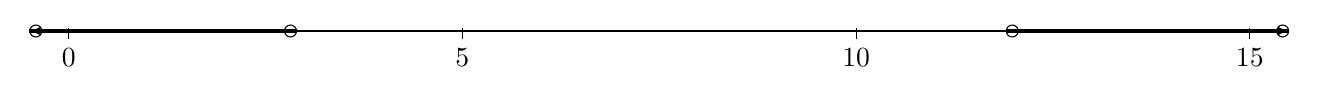
\begin{tikzpicture}
        \draw[latex-] (-0.5,0) -- (15.5,0) ;
        \draw[-latex] (-0.5,0) -- (15.5,0) ;
        \foreach \x in  {0, 5, 10, 15}
        \draw[shift={(\x,0)},color=black] (0pt,1pt) -- (0pt,-3pt);
        \foreach \x in  {0, 5, 10, 15}
        \draw[shift={(\x,0)},color=black] (0pt,0pt) -- (0pt,-3pt) node[below]
            {$\x$};
        \draw[o-o] (11.9,0) -- (15.5,0);
        \draw[very thick    ](11.9,0) -- (15.5,0);
        \draw[o-o] (-0.5,0) -- (2.9,0);
        \draw[very thick    ] (-0.5,0) -- (2.9,0);
    \end{tikzpicture}
    \begin{align*}
        \boxed{(-\infty, 3)\cup(12, \infty)}
    \end{align*}

    \subsection*{413}
    \begin{align*}
        2(x + 3 ) &\geq 0 \hspace{2cm} or &3(x + 4)  &\leq 6 \\
        2x + 6 & \geq 0 &3x + 12 & \leq 6 \\
        2x \cancel{+ 6} &\geq 0 - 6 &3x \cancel{+ 12} & \leq 6 - 12 \\
        2x &\geq -6 &3x &\leq -6 \\
        \frac{2x}{2} &\geq \frac{-6}{2} &\frac{3x}{3} &\leq \frac{-6}{3} \\
        x &\geq -3 & x &\leq -2
    \end{align*}
    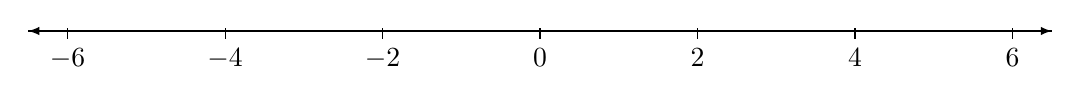
\begin{tikzpicture}
        \draw[latex-] (-6.5,0) -- (6.5,0) ;
        \draw[-latex] (-6.5,0) -- (6.5,0) ;
        \foreach \x in {-6,-4,-2,0,2,4,6}
        \draw[shift={(\x,0)},color=black] (0pt,1pt) -- (0pt,-3pt);
        \foreach \x in {-6,-4,-2,0,2,4,6}
        \draw[shift={(\x,0)},color=black] (0pt,0pt) -- (0pt,-3pt) node[below]
            {$\x$};
    \end{tikzpicture}
    \begin{align*}
        \boxed{(-\infty, \infty)}
    \end{align*}

    \subsection*{415}
    \begin{align*}
        \frac{3}{4}x + 2 &\leq -1 \hspace{2cm} or &\frac{1}{2}(x + 8)  &\geq -3 \\
        4(\frac{3}{4}x + 2) &\leq 4 \times -1  &2 \times \frac{1}{2}(x + 8)  &\geq 2 \times -3\\
        3x + 8 &\leq -4 &x + 8 &\geq -6 \\
        3x \cancel{+ 8} &\leq -4 - 8 &x \cancel{+ 8} &\geq -6 - 8 \\
        3x &\leq -12 &x &\geq -14 \\
        \frac{3x}{3} &\leq \frac{-12}{3} &x &\geq -14 \\
        x &\leq -4 &x &\geq -14 \\
    \end{align*}
    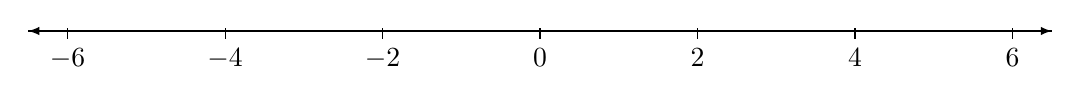
\begin{tikzpicture}
        \draw[latex-] (-6.5,0) -- (6.5,0) ;
        \draw[-latex] (-6.5,0) -- (6.5,0) ;
        \foreach \x in {-6,-4,-2,0,2,4,6}
        \draw[shift={(\x,0)},color=black] (0pt,1pt) -- (0pt,-3pt);
        \foreach \x in {-6,-4,-2,0,2,4,6}
        \draw[shift={(\x,0)},color=black] (0pt,0pt) -- (0pt,-3pt) node[below]
            {$\x$};
    \end{tikzpicture}
    \begin{align*}
        \boxed{(-\infty,\infty)}
    \end{align*}


    \subsection*{415}
    \begin{align*}
        \frac{3}{4}x + 2 &\leq -1 \hspace{2cm} or &\frac{1}{2}(x + 8)  &\geq -3 \\
        4(\frac{3}{4}x + 2) &\leq 4 \times -1  &2 \times \frac{1}{2}(x + 8)  &\geq 2 \times -3\\
        3x + 8 &\leq -4 &x + 8 &\geq -6 \\
        3x \cancel{+ 8} &\leq -4 - 8 &x \cancel{+ 8} &\geq -6 - 8 \\
        3x &\leq -12 &x &\geq -14 \\
        \frac{3x}{3} &\leq \frac{-12}{3} &x &\geq -14 \\
        x &\leq -4 &x &\geq -14 \\
    \end{align*}
    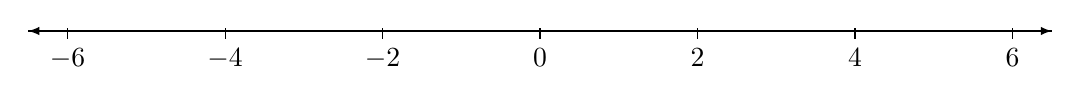
\begin{tikzpicture}
        \draw[latex-] (-6.5,0) -- (6.5,0) ;
        \draw[-latex] (-6.5,0) -- (6.5,0) ;
        \foreach \x in {-6,-4,-2,0,2,4,6}
        \draw[shift={(\x,0)},color=black] (0pt,1pt) -- (0pt,-3pt);
        \foreach \x in {-6,-4,-2,0,2,4,6}
        \draw[shift={(\x,0)},color=black] (0pt,0pt) -- (0pt,-3pt) node[below]
            {$\x$};
    \end{tikzpicture}
    \begin{align*}
        \boxed{(-\infty,\infty)}
    \end{align*}


    \subsection*{417}
    \begin{align*}
        6(2x -1) &> 6 \hspace{2cm} and &2x + 3 &\geq 0 \\
        12x - 6 &> 6  &2x + 3 &\geq 0 \\
        12x \cancel{- 6} &> 6 + 6  &2x \cancel{+ 3} &\geq 0 - 3 \\
        12x  &> 12  &2x  &\geq - 3 \\
        \frac{12x}{12}  &> \frac{12}{12}  &\frac{2x}{2}  &\geq - \frac{3}{2} \\
        x &> 1 &x &\geq \frac{3}{2} \\
        &\hspace{2cm} x > 1
    \end{align*}
    \begin{tikzpicture}
        \draw[latex-] (-6.5,0) -- (6.5,0) ;
        \draw[-latex] (-6.5,0) -- (6.5,0) ;
        \foreach \x in  {-6,-4,-2,0,2,4,6}
        \draw[shift={(\x,0)},color=black] (0pt,3pt) -- (0pt,-3pt);
        \foreach \x in {-6,-4,-2,0,2,4,6}
        \draw[shift={(\x,0)},color=black] (0pt,0pt) -- (0pt,-3pt) node[below]
            {$\x$};
        \draw[o-o] (1.1,0) -- (6.5,0);
        \draw[very thick    ](1.1,0) -- (6.5,0);
    \end{tikzpicture}
    \begin{align*}
        \boxed{(1, \infty)}
    \end{align*}

    \subsection*{419}
    \begin{align*}
        \frac{1}{2}x - 5 &\leq 3 \hspace{2cm} or &\frac{1}{4}(x - 8)  &\geq -3 \\
        2(\frac{1}{2}x - 5) &\leq 2\times 3 & 4 \times \frac{1}{4}(x - 8)  &\geq 4 \times -3 \\
        x - 5 &\leq 6 &4(x - 8)  &\geq -12\\
        x - 5 &\leq 6 &4x - 32  &\geq -12\\
        x \cancel{- 5} &\leq 6 + 5 &4x \cancel{- 32}  &\geq -12 + 32\\
        x & \leq 11 &4x & \geq 20\\
        &&\frac{4x}{4} & \geq \frac{20}{4} \\
        x & \leq 11 &x & \geq 5\\
    \end{align*}
    \begin{tikzpicture}
        \draw[latex-] (-6.5,0) -- (6.5,0) ;
        \draw[-latex] (-6.5,0) -- (6.5,0) ;
        \foreach \x in {-6,-4,-2,0,2,4,6}
        \draw[shift={(\x,0)},color=black] (0pt,1pt) -- (0pt,-3pt);
        \foreach \x in {-6,-4,-2,0,2,4,6}
        \draw[shift={(\x,0)},color=black] (0pt,0pt) -- (0pt,-3pt) node[below]
            {$\x$};
    \end{tikzpicture}
    \begin{align*}
        \boxed{(-\infty,\infty)}
    \end{align*}

    \subsection*{421}
    \begin{align*}
        \frac{1}{5}(x - 5) + 6 &< 4\hspace{2cm} and &3 - \frac{2}{3}x &< 5 \\
        5 \times (\frac{1}{5}(x - 5) + 6) &\< 5 \times 4 &3 \times (3 - \frac{2}{3}x) &< 3 \times 5  \\
        x - 5 + 30 &< 20 &9 - 2x &< 15  \\
        x  + 25 &< 20   \\
        x  \cancel{+ 25} &< 20 - 25 &\cancel{9} - 2x &< 15 - 9  \\
        x  &< -5 & - 2x &< 6  \\
        && \frac{-2x}{-2} &< \frac{6}{-2}\\
        x  &< -5  &x &>-3 \\
    \end{align*}
    \begin{tikzpicture}
        \draw[latex-] (-6.5,0) -- (6.5,0) ;
        \draw[-latex] (-6.5,0) -- (6.5,0) ;
        \foreach \x in  {-6,-4,-2,0,2,4,6}
        \draw[shift={(\x,0)},color=black] (0pt,3pt) -- (0pt,-3pt);
        \foreach \x in {-6,-4,-2,0,2,4,6}
        \draw[shift={(\x,0)},color=black] (0pt,0pt) -- (0pt,-3pt) node[below]
            {$\x$};
    \end{tikzpicture}
    \begin{align*}
        \boxed{No Solutions}
    \end{align*}

    \subsection*{423}
    \begin{align*}
        6x -3 &\leq 1\hspace{2cm} and &5x - 1 &> -6 \\
        6x \cancel{-3} &\leq 1+3 &5x \cancel{- 1} &> -6 + 1 \\
        6x &\leq 4 &5x &> -5  \\
        \frac{6x}{6} &\leq \frac{4}{6} &\frac{5x}{5} &> \frac{-5}{5}  \\
        x &\leq \frac{4}{6} &x &> -1  \\
        x &\leq \frac{2}{3} &x &> -1  \\
        &\hspace{2cm} -1 < x \leq \frac{2}{3} \\
    \end{align*}
    \begin{tikzpicture}
        \draw[latex-] (-6.5,0) -- (6.5,0) ;
        \draw[-latex] (-6.5,0) -- (6.5,0) ;
        \foreach \x in  {-6,-4,-2,0,2,4,6}
        \draw[shift={(\x,0)},color=black] (0pt,3pt) -- (0pt,-3pt);
        \foreach \x in {-6,-4,-2,0,2,4,6}
        \draw[shift={(\x,0)},color=black] (0pt,0pt) -- (0pt,-3pt) node[below]
            {$\x$};
        \draw[o-*] (-1.1,0) -- (0.66,0);
        \draw[very thick    ](-1.1,0) -- (0.66,0);
    \end{tikzpicture}
    \begin{align*}
        \boxed{[-1, \frac{2}{3})}
    \end{align*}

    \subsection*{425}
    \begin{align*}
        -5 &\leq 3x -2 \leq 4 \\
        -5 + 2 &\leq 3x \cancel{-2} \leq 4 + 2\\
        -3 &\leq 3x \leq 6\\
        &\hspace{-.5cm}\frac{-3 \leq 3x \leq 6}{3}\\
        -1 &\leq x \leq 2\\
    \end{align*}
    \begin{tikzpicture}
        \draw[latex-] (-6.5,0) -- (6.5,0) ;
        \draw[-latex] (-6.5,0) -- (6.5,0) ;
        \foreach \x in  {-6,-4,-2,0,2,4,6}
        \draw[shift={(\x,0)},color=black] (0pt,3pt) -- (0pt,-3pt);
        \foreach \x in {-6,-4,-2,0,2,4,6}
        \draw[shift={(\x,0)},color=black] (0pt,0pt) -- (0pt,-3pt) node[below]
            {$\x$};
        \draw[*-*] (-1.1,0) -- (2.1,0);
        \draw[very thick    ](-1.1,0) -- (2.1,0);
    \end{tikzpicture}
    \begin{align*}
        \boxed{[-1, 2]}
    \end{align*}

    \section*{2.7 Part 1, 435 to 455 odd}
    \subsection*{435 a}
    \begin{align*}
        &|x| = 4 \\
        &\boxed{x = 4, x = -4}
    \end{align*}

    \subsection*{435 b}
    \begin{align*}
        &|y| = -5 \\
        &\boxed{No Solution}
    \end{align*}

    \subsection*{435 c}
    \begin{align*}
        &|z| = 0 \\
        &\boxed{z = 0}
    \end{align*}

    \subsection*{437 a}
    \begin{align*}
        &|x| = 3 \\
        &\boxed{x = 3,x = -3}
    \end{align*}

    \subsection*{437 b}
    \begin{align*}
        &|y| = -1 \\
        &\boxed{No Solution}
    \end{align*}

    \subsection*{437 c}
    \begin{align*}
        &|z| = 0 \\
        &\boxed{z = 0}
    \end{align*}


    \subsection*{439}
    \begin{align*}
        |4x - 1| -3 &= 0 \\
        |4x - 1| \cancel{-3} &= 0 + 3 \\
        |4x - 1| &= 3 \\
    \end{align*}
    \begin{align*}
        4x - 1 &= 3 &4x - 1 &= -3\\
        4x \cancel{- 1} &= 3 + 1 &4x \cancel{- 1} &= -3 + 1\\
        4x  &=  4 &4x  &= -2\\
        \frac{4x}{4}  &=  \frac{4}{4} &\frac{4x}{4}  &= \frac{-2}{4}\\
        x &= 1  &x &= -\frac{1}{2}\\
    \end{align*}
    \begin{align*}
        \boxed{x = 1, x = -\frac{1}{2}}
    \end{align*}

    \subsection*{441}
    \begin{align*}
        |4x +7| +2 &= 5 \\
        |4x +7| \cancel{+2} &= 5 - 2 \\
        |4x +7|  &= 3 \\
    \end{align*}
    \begin{align*}
        4x +7 &= 3 &4x +7 &= -3\\
        4x \cancel{+ 7} &= 3 -7 &4x \cancel{+ 7} &= -3 -7\\
        4x  &=  -4 &4x  &= -10\\
        \frac{4x}{4}  &=  -\frac{4}{4} &\frac{4x}{4}  &= -\frac{10}{4}\\
        x &= -1  &x &= -\frac{5}{2}\\
    \end{align*}
    \begin{align*}
        \boxed{x = -1, x = -\frac{5}{2}}
    \end{align*}

    \subsection*{443}
    \begin{align*}
        3|x -4| +2 &= 11 \\
        3|x -4| \cancel{+2} &= 11 - 2 \\
        3|x -4|  &= 9 \\
        \frac{3|x -4|}{3}  &= \frac{9}{3} \\
        |x - 4| &= 3
    \end{align*}
    \begin{align*}
        x - 4 &= 3 &x -4 &= -3\\
        x \cancel{- 4} &= 3 +4 &x \cancel{-4} &= -3 +4\\
        x  &=  7 &x  &= 1\\
    \end{align*}
    \begin{align*}
        \boxed{x = 7, x = 1}
    \end{align*}

    \subsection*{445}
    \begin{align*}
        3|x +2| -5 &= 4 \\
        3|x +2| \cancel{-5} &= 4 + 5 \\
        3|x +2|  &= 9 \\
        \frac{3|x +2|}{3}  &= \frac{9}{3} \\
        |x +2| &= 3
    \end{align*}
    \begin{align*}
        x + 2 &= 3 &x +2 &= -3\\
        x \cancel{+2} &= 3 -2 &x \cancel{+2} &= -3 -2\\
        x  &=  1 &x  &= -1\\
    \end{align*}
    \begin{align*}
        \boxed{x = 1, x = -5}
    \end{align*}


    \subsection*{447}
    \begin{align*}
        -3|x -4| +4 &= -5 \\
        -3|x -4| \cancel{+4} &= -5 - 4 \\
        -3|x -4| &= -9 \\
        \frac{-3|x -4|}{-3}  &= \frac{-9}{-3} \\
        |x - 4| &= 3
    \end{align*}
    \begin{align*}
        x - 4 &= 3 &x -4 &= -3\\
        x \cancel{-4} &= 3 + 4 &x \cancel{-4} &= -3 + 4\\
        x  &=  7 &x  &= 1\\
    \end{align*}
    \begin{align*}
        \boxed{x = 7, x = 1}
    \end{align*}


    \subsection*{449}
    \begin{align*}
        |\frac{3}{5}x -2| +5 &= 2 \\
        |\frac{3}{5}x -2| \cancel{+5} &= 2 - 5 \\
        |\frac{3}{5}x -2| &= -3 \\
        |\frac{3}{5}x -2| &= \boxed{-3} \\
    \end{align*}
    \begin{align*}
        \boxed{No Solution}
    \end{align*}

    \subsection*{451}
    \begin{align*}
        |\frac{1}{4x} +3| + 3 &= 1 \\
        |\frac{1}{4x} +3| \cancel{+ 3} &= 1 - 3 \\
        |\frac{1}{4x} +3| &= -2\\
        |\frac{1}{4x} +3| &= \boxed{-2}\\
    \end{align*}
    \begin{align*}
        \boxed{No Solution}
    \end{align*}


    \subsection*{453}
    \begin{align*}
        |4x + 3| &= |2x + 1| \\
    \end{align*}
    \begin{align*}
        4x + 3 &= -2x - 1 &4x + 3 &= 2x + 1\\
        4x \cancel{+ 3} &= -2x - 1 - 3 &4x \cancel{+3} &= 2x + 1 -3\\
        4x  &=  -2x - 4 &4x  &= 2x - 2\\
        4x  +2x &=  \cancel{-2x} - 4 &4x -2x &= \cancel{2x} - 2\\
        6x & = -4 &2x &= -2\\
        \frac{6x}{6} &= \frac{-4}{6} &\frac{2x}{2} &= \frac{-2}{2} \\
        x &= -\frac{2}{3} &x &=-1\\
    \end{align*}
    \begin{align*}
        \boxed{x = -\frac{2}{3}\hspace{.2cm}or\hspace{.2cm}  x = -1}
    \end{align*}

    \subsection*{455}
    \begin{align*}
        |6 - x| &= |3 - 2x| \\
    \end{align*}
    \begin{align*}
        6 - x &= 3 - 2x &6 - x &= -3 + 2x\\
        -x \cancel{+ 6} &= -2x + 3 -6 &-x \cancel{+6} &= 2x -3 - 6\\
        -x  &=  -2x - 3 &-x  &= 2x - 9\\
        -x + 2x  &=  \cancel{-2x} - 3 &-x - 2x &= \cancel{2x} - 9\\
        x &= -3 &-3x &=-9\\
        &&\frac{-3x}{-3} &= \frac{-9}{-3} \\
        x &= -3 &x &=3\\
    \end{align*}
    \begin{align*}
        \boxed{x = -3\hspace{.2cm}or\hspace{.2cm}  x = 3}
    \end{align*}

    \section*{2.7 Part 2, 469 to 479 odd}
    \subsection*{469}
    \begin{align*}
        |x| > 6
    \end{align*}
    \hspace{-1.5cm}
    \begin{tikzpicture}
        \draw[latex-] (-8.5,0) -- (8.5,0) ;
        \draw[-latex] (-8.5,0) -- (8.5,0) ;
        \foreach \x in  {-8,-4,0,4,8}
        \draw[shift={(\x,0)},color=black] (0pt,3pt) -- (0pt,-3pt);
        \foreach \x in  {-8,-4,0,4,8}
        \draw[shift={(\x,0)},color=black] (0pt,0pt) -- (0pt,-3pt) node[below]
            {$\x$};
        \draw[o-o] (6,0) -- (8.5,0);
        \draw[very thick    ](6,0) -- (8.5,0);
        \draw[o-o] (-8.5,0) -- (-6,0);
        \draw[very thick    ](-8.5,0) -- (-6,0);
    \end{tikzpicture}
    \begin{align*}
        \boxed{(-\infty, -6)\cup(6, \infty)}
    \end{align*}


    \subsection*{471}
    \begin{align*}
        |x| \geq 5
    \end{align*}
    \hspace{-1.5cm}
    \begin{tikzpicture}
        \draw[latex-] (-8.5,0) -- (8.5,0) ;
        \draw[-latex] (-8.5,0) -- (8.5,0) ;
        \foreach \x in  {-8,-4,0,4,8}
        \draw[shift={(\x,0)},color=black] (0pt,3pt) -- (0pt,-3pt);
        \foreach \x in  {-8,-4,0,4,8}
        \draw[shift={(\x,0)},color=black] (0pt,0pt) -- (0pt,-3pt) node[below]
            {$\x$};
        \draw[*-o] (5,0) -- (8.5,0);
        \draw[very thick    ](5,0) -- (8.5,0);
        \draw[o-*] (-8.5,0) -- (-5,0);
        \draw[very thick    ](-8.5,0) -- (-5,0);
    \end{tikzpicture}
    \begin{align*}
        \boxed{(-\infty, -5]\cup[5, \infty)}
    \end{align*}



    \subsection*{473}
    \begin{align*}
        |x - 5| &> -2\\
        |x - 5| &> \boxed{-2}
    \end{align*}
    \hspace{-1.5cm}
    \begin{tikzpicture}
        \draw[latex-] (-8.5,0) -- (8.5,0) ;
        \draw[-latex] (-8.5,0) -- (8.5,0) ;
        \foreach \x in  {-8,-4,0,4,8}
        \draw[shift={(\x,0)},color=black] (0pt,3pt) -- (0pt,-3pt);
        \foreach \x in  {-8,-4,0,4,8}
        \draw[shift={(\x,0)},color=black] (0pt,0pt) -- (0pt,-3pt) node[below]
            {$\x$};
    \end{tikzpicture}
    \begin{align*}
        \boxed{(-\infty, \infty)}
    \end{align*}

    \subsection*{475}
    \begin{align*}
        |2x - 1| > 5
    \end{align*}
    \begin{align*}
        2x - 1 &> 5 &2x - 1 &< -5 \\
        2x \cancel{- 1} &> 5 + 1 &2x \cancel{- 1} &< -5 + 1 \\
        2x  &> 6 &2x  &< -4 \\
        \frac{2x}{2}  &> \frac{6}{2} &\frac{2x}{2}  &< \frac{-4}{2} \\
        x &> 3 &x  &< -2 \\
    \end{align*}
    \hspace{-1.5cm}
    \begin{tikzpicture}
        \draw[latex-] (-8.5,0) -- (8.5,0) ;
        \draw[-latex] (-8.5,0) -- (8.5,0) ;
        \foreach \x in  {-8,-4,0,4,8}
        \draw[shift={(\x,0)},color=black] (0pt,3pt) -- (0pt,-3pt);
        \foreach \x in  {-8,-4,0,4,8}
        \draw[shift={(\x,0)},color=black] (0pt,0pt) -- (0pt,-3pt) node[below]
            {$\x$};
        \draw[o-o] (3,0) -- (8.5,0);
        \draw[very thick    ](3,0) -- (8.5,0);
    \end{tikzpicture}
    \begin{align*}
        \boxed{(-\infty, -2)\cup(3, \infty)}
    \end{align*}

    \subsection*{477}
    \begin{align*}
        |x - 7| \geq 1
    \end{align*}
    \begin{align*}
        x - 7 &\geq 1 &x - 7 &\leq -1 \\
        x \cancel{- 7} &\geq 1 + 7 &x \cancel{- 7} &\leq -1 + 7\\
        x  &\geq 8 &x  &\leq 6 \\
    \end{align*}
    \hspace{-4.5cm}
    \begin{tikzpicture}
        \draw[latex-] (-10.5,0) -- (10.5,0) ;
        \draw[-latex] (-10.5,0) -- (10.5,0) ;
        \foreach \x in  {-10,-5,0,5,10}
        \draw[shift={(\x,0)},color=black] (0pt,3pt) -- (0pt,-3pt);
        \foreach \x in  {-10,-5,0,5,10}
        \draw[shift={(\x,0)},color=black] (0pt,0pt) -- (0pt,-3pt) node[below]
            {$\x$};
        \draw[*-o] (8,0) -- (10.5,0);
        \draw[very thick    ](8,0) -- (10.5,0);
        \draw[o-*] (-10.6,0) -- (6,0);
        \draw[very thick    ](-10.6,0) -- (6,0);
    \end{tikzpicture}
    \begin{align*}
        \boxed{(-\infty, 6]\cup[8, \infty)}
    \end{align*}

    \subsection*{479}
    \begin{align*}
        5|x|+ 6 &\geq 1 \\
        5|x|\cancel{+ 6} &\geq 1 - 6 \\
        5|x| &\geq -5 \\
        \frac{5|x|}{5} &\geq \frac{-5}{5} \\
        |x| &\geq -1\\
        |x| &\geq \boxed{-1}
    \end{align*}
    \hspace{-1.5cm}
    \begin{tikzpicture}
        \draw[latex-] (-8.5,0) -- (8.5,0) ;
        \draw[-latex] (-8.5,0) -- (8.5,0) ;
        \foreach \x in  {-8,-4,0,4,8}
        \draw[shift={(\x,0)},color=black] (0pt,3pt) -- (0pt,-3pt);
        \foreach \x in  {-8,-4,0,4,8}
        \draw[shift={(\x,0)},color=black] (0pt,0pt) -- (0pt,-3pt) node[below]
            {$\x$};
    \end{tikzpicture}
    \begin{align*}
        \boxed{(-\infty, \infty)}
    \end{align*}

\end{document}
